\chapter{The Theory of \texorpdfstring{$L$}{L}-functions}
  We start our discussion of $L$-functions with Dirichlet series. Dirichlet series are essential tools in analytic number theory because they are a way of analytically encoding arithmetic information. If the Dirichlet series possesses special properties we call it an $L$-function. From the analytic properties of $L$-functions we can extract number theoretic results. After discussing Dirichlet series we will define $L$-functions and their associated data. The material following the data of $L$-functions consists of many important discussions about the analytic properties of $L$-functions: the approximate functional equation, the Riemann hypothesis and Lindel\"of hypothesis, the central value, logarithmic derivatives, zero density, zero-free regions, and explicit formulas.
  \section{Dirichlet Series}
    A \textbf{Dirichlet series}\index{Dirichlet series} $D(s)$ is a sum of the form
    \[
      D(s) = \sum_{n \ge 1}\frac{a(n)}{n^{s}},
    \]
    with $a(n) \in \C$. We exclude the case $a(n) = 0$ for all $n \ge 1$ so that $D(s)$ is not identically zero. We would first like to understand where this series converges. It does not take much for $D(s)$ to converge uniformly in a sector:

    \begin{theorem}\label{thm:convergence_of_Dirichlet_series}
      Suppose $D(s)$ is a Dirichlet series that converges at $s_{0} = \s_{0}+it_{0}$. Then for any $H > 0$, $D(s)$ converges uniformly in the sector
      \[
        \{s \in \C:\text{$\s \ge \s_{0}$ and $|t-t_{0}| \le H(\s-\s_{0})$}\}.
      \]
    \end{theorem}
    \begin{proof}
      Set $R(u) = \sum_{n \ge u}\frac{a(n)}{n^{-s_{0}}}$ so that $a(n) = (R(n)-R(n+1))n^{s_{0}}$. Then for any two positive integers $N$ and $M$ with $1 \le M < N$, partial summation (see \cref{append:Summation_Formulas}) implies
      \begin{equation}\label{equ:convergence_of_Dirichlet_series_1}
        \sum_{M \le n \le N}\frac{a(n)}{n^{s}} = R(M)M^{s_{0}-s}-R(N)N^{s_{0}-s}-\sum_{M+1 \le n \le N}R(n)((n-1)^{s_{0}-s}-n^{s_{0}-s}).
      \end{equation}
      We will now express the sum on the right-hand side as an integral. To do this, observe that
      \[
        (n-1)^{s_{0}-s}-n^{s_{0}-s} = -(s_{0}-s)\int_{n-1}^{n}u^{s_{0}-s-1}\,du.
      \]
      Therefore
      \begin{equation}\label{equ:convergence_of_Dirichlet_series_2}
        \begin{aligned}
          \sum_{M+1 \le n \le N}R(n)((n-1)^{s_{0}-s}-n^{s_{0}-s}) &= -(s_{0}-s)\sum_{M+1 \le n \le N}R(n)\int_{n-1}^{n}u^{s_{0}-s-1}\,du \\
          &= -(s_{0}-s)\sum_{M+1 \le n \le N}\int_{n-1}^{n}R(u)u^{s_{0}-s-1}\,du \\
          &= -(s_{0}-s)\int_{M}^{N}R(u)u^{s_{0}-s-1}\,du,
        \end{aligned}
      \end{equation}
      where the second to last line follows because $R(u)$ is constant on the interval $[u,u+1)$. Combining \cref{equ:convergence_of_Dirichlet_series_1,equ:convergence_of_Dirichlet_series_2} gives
      \begin{equation}\label{equ:convergence_of_Dirichlet_series_3}
        \sum_{M \le n \le N}\frac{a(n)}{n^{s}} = R(M)M^{s_{0}-s}-R(N)N^{s_{0}-s}+(s_{0}-s)\int_{M}^{N}R(u)u^{s_{0}-s-1}\,du.
      \end{equation}
      Now there exists an $M$ such that $|R(u)| < \e$ for all $u \ge M$ because $D(s)$ is convergent at $s_{0}$. In particular, $|R(u)u^{s_{0}-s}| < \e$ for all $u \ge M$ because $\s \ge \s_{0}$. Moreover for $s$ in the prescribed sector,
      \[
        |s-s_{0}| \le (\s-\s_{0})+|t-t_{0}| \le (H+1)(\s-\s_{0}).
      \]
      These estimates and \cref{equ:convergence_of_Dirichlet_series_3} together imply
      \[
        \left|\sum_{M \le n \le N}\frac{a(n)}{n^{s}}\right| \le 2\e+\e|s-s_{0}|\int_{M}^{N}u^{\s_{0}-\s-1}\,du \le 2\e+\e(H+1)(\s-\s_{0})\int_{M}^{N}u^{\s_{0}-\s-1}\,du.
      \]
      Since the integral is finite, $\sum_{M \le n \le N}\frac{a(n)}{n^{s}}$ can be made arbitrarily small uniformly for $s$ in the desired sector. The claim now follows by the uniform version of Cauchy's criterion.
    \end{proof}
    
    By taking $H \to \infty$ in \cref{thm:convergence_of_Dirichlet_series} we see that $D(s)$ converges in the region $\s > \s_{0}$. Let $\s_{c}$ be the infimum of all $\s$ for which $D(s)$ converges. We call $\s_{c}$ the \textbf{abscissa of convergence}\index{abscissa of convergence} of $D(s)$. Similarly, let $\s_{a}$ be the infimum of all $\s$ for which $D(s)$ converges absolutely. Since the terms of $D(s)$ are holomorphic, the convergence is locally absolutely uniform (actually uniform in sectors) for $\s > \s_{a}$. It follows that $D(s)$ is holomorphic in the region $\s > \s_{a}$.  We call $\s_{a}$ the \textbf{abscissa of absolute convergence}\index{abscissa of absolute convergence} of $D(s)$. One should think of $\s_{c}$ and $\s_{a}$ as the boundaries of convergence and absolute convergence respectively. Of course, anything can happen at $\s = \s_{c}$ and $\s = \s_{a}$, but to the right of these lines we have convergence and absolute convergence of $D(s)$ respectively. It turns out that $\s_{a}$ is never far from $\s_{c}$ provided $\s_{c}$ is finite:

    \begin{theorem}
      If $D(s)$ is a Dirichlet series with finite abscissa of convergence $\s_{c}$, then
      \[
        \s_{c} \le \s_{a} \le \s_{c}+1.
      \]
    \end{theorem}
    \begin{proof}
      The first inequality is trivial since absolute convergence implies convergence. For the second inequality, since $D(s)$ converges at $\s_{c}+\e$, the terms $a(n)n^{-(\s_{c}+\e)}$ tend to zero as $n \to \infty$. Therefore $a(n) \ll_{\e} n^{\s_{c}+\e}$ where the implicit constant is independent of $n$. But then $a(n)n^{-(\s_{c}+\e)} \ll_{\e} 1$ which implies $\sum_{n \ge 1}a(n)n^{-(\s_{c}+1+2\e)}$ is absolutely convergent by the comparison test with respect to $\sum_{n \ge 1}n^{-(1+\e)}$. In terms of $D(s)$, this means $\s_{a} \le \s_{c}+1+2\e$ and taking $\e \to 0$ gives the second inequality.
    \end{proof}

    We will now introduce several convergence theorems for Dirichlet series. It will be useful to setup some notation first. If $D(s)$ is a Dirichlet series with coefficients $a(n)$, then for $X > 0$, we set
    \[
      A(X) = \sum_{n \le X}a(n) \quad \text{and} \quad |A|(X) = \sum_{n \le X}|a(n)|.
    \]
    These are the partial sums of the coefficients $a(n)$ and $|a(n)|$ up to $X$ respectively. Our first convergence theorem relates boundedness of $A(X)$ to the value of $\s_{c}$: 
    
    \begin{proposition}\label{prop:Dirichlet_series_convergence_bounded_coefficient_sum}
      Suppose $D(s)$ is a Dirichlet series and that $A(X) \ll 1$. Then $\s_{c} \le 0$.
    \end{proposition}
    \begin{proof}
      Let $s$ be such that $\s > 0$. Since $A(X) \ll 1$, $A(X)X^{-s} \to 0$ as $X \to \infty$. Abel's summation formula (see \cref{append:Summation_Formulas}) then implies
      \[
        D(s) = s\int_{1}^{\infty}A(u)u^{-(s+1)}\,du.
      \]
      But because $A(u) \ll 1$, we have
      \[
        s\int_{1}^{\infty}A(u)u^{-(s+1)}\,du \ll s\int_{1}^{\infty}u^{-(\s+1)}\,du = -\frac{s}{\s}u^{-\s}\bigg|_{1}^{\infty} = \frac{s}{\s},
      \]
      and so the integral converges for $\s > 0$. Thus $D(s)$ converges for $\s > 0$ and therefore $\s_{c} \le 0$.
    \end{proof}

    Our next theorem states that if the coefficients of $D(s)$ are of polynomial growth, we can obtain an upper bound for the abscissa of absolute convergence:

    \begin{proposition}\label{prop:Dirichlet_series_convergence_polynomial_bound}
      Suppose $D(s)$ is a Dirichlet series whose coefficients satisfy $a(n) \ll_{\a} n^{\a}$ for some real $\a$. Then the abscissa of absolute convergence satisfies $\s_{a} \le 1+\a$.
    \end{proposition}
    \begin{proof}
      It suffices to show that $D(s)$ is absolutely convergent in the region $\s > 1+\a$. For $s$ is in this region, the polynomial bound gives
      \[
        D(s) \ll \sum_{n \ge 1}\left|\frac{a(n)}{n^{s}}\right| \ll_{\a} \sum_{n \ge 1}\frac{1}{n^{\s-\a}}.
      \]
      The latter series converges by the integral test because $\s-\a > 1$. Therefore $D(s)$ is absolutely convergent.
    \end{proof}

    Obtaining polynomial bounds on coefficients of Dirichlet series are, in most cases, not hard to establish. So the assumption in \cref{prop:Dirichlet_series_convergence_polynomial_bound} is mild. Actually, there is a partial converse to \cref{prop:Dirichlet_series_convergence_polynomial_bound} which gives an approximate size to $A(X)$:

    \begin{proposition}\label{prop:Dirichlet_series_coefficient_size_on_average}
      Suppose $D(s)$ is a Dirichlet series with finite and nonnegative abscissa of absolute convergence $\s_{a}$. Then
      \[
        A(X) \ll_{\e} X^{\s_{a}+\e}.
      \]
    \end{proposition}
    \begin{proof}
      By Abel's summation formula (see \cref{append:Summation_Formulas}),
      \begin{equation}\label{prop:Dirichlet_series_coefficient_size_on_average_1}
        \sum_{n \le X}\frac{a(n)}{n^{\s_{a}+\e}} = A(X)X^{-(\s_{a}+\e)}+(\s_{a}+\e)\int_{0}^{X}A(u)u^{-(\s_{a}+\e+1)}\,du.
      \end{equation}
      If we set $R(u) = \sum_{n \ge u}\frac{a(n)}{n^{\s_{a}+\e}}$, then $a(n) = (R(n)-R(n+1))n^{\s_{a}+\e}$ and it follows that
      \[
        A(u) = \sum_{n \le u}(R(n)-R(n+1))n^{\s_{a}+\e}.
      \]
      Substituting this into \cref{prop:Dirichlet_series_coefficient_size_on_average_1}, we obtain
      \[
        \int_{0}^{X}\sum_{n \le u}(R(n)-R(n+1))n^{\s_{a}+\e}u^{-(\s_{a}+\e+1)}\,du.
      \]
      As $R(n)$ is constant on the interval $[n,n+1)$, linearity of the integral implies
      \[
        \int_{0}^{X}\sum_{n \le u}(R(n)-R(n+1))n^{\s_{a}+\e}u^{-(\s_{a}+\e+1)}\,du = \sum_{0 \le n \le X}(R(n)-R(n+1))n^{\s_{a}+\e}\int_{n}^{n+1}u^{-(\s_{a}+\e+1)}+O_{\e}(1),
      \]
      where the $O$-estimate is present since $X$ may not be an integer. Now $R(n) \ll_{\e} 1$ since it is the tail of $D(\s_{a}+\e)$ and moreover,
      \[
        \int_{n}^{n+1}u^{-(\s_{a}+\e+1)} = -\frac{u^{-(\s_{a}+\e)}}{\s_{a}+\e}\bigg|_{n}^{n+1} = \frac{n^{-(\s_{a}+\e)}}{\s_{a}+\e}-\frac{(n+1)^{-(\s_{a}+\e)}}{\s_{a}+\e} \ll_{\e} 1,
      \]
      because $\s_{a}+\e > 0$. So
      \[
        \int_{0}^{X}A(u)u^{-(\s_{a}+\e+1)}\,du = \int_{0}^{X}\sum_{n \le u}(R(n)-R(n+1))n^{\s_{a}+\e}u^{-(\s_{a}+\e+1)}\,du \ll_{\e} 1.
      \]
      Also, $\sum_{n \le X}\frac{a(n)}{n^{\s_{a}+\e}} \ll_{\e} 1$ because $D(\s_{a}+\e)$ converges. We conclude
      \[
        A(X)X^{-(\s_{a}+\e)} = \sum_{n \le X}\frac{a(n)}{n^{\s_{a}+\e}}-(\s_{a}+\e)\int_{0}^{X}A(u)u^{-(\s_{a}+\e+1)}\,du. \ll_{\e} 1,
      \]
      which is equivalent to the desired estimate.
    \end{proof}

    A way to think about \cref{prop:Dirichlet_series_coefficient_size_on_average} is that if the abscissa of absolute convergence is $\s_{a} \ge 0$ then the size of the coefficients $a(n)$ is at most $n^{\s_{a}+\e}$ on average. Of corse, if $a(n) \ll_{\a} n^{\a}$ then \cref{prop:Dirichlet_series_convergence_polynomial_bound} implies that $\s_{a} \le 1+\a$ and so \cref{prop:Dirichlet_series_coefficient_size_on_average} gives the significantly weaker estimate $A(X) \ll_{\e} X^{1+\a+\e}$. However, if we have a bound of the form $|A|(X) \ll_{\a} X^{\a}$ we can still obtain an upper estimate for the abscissa of absolute convergence:

    \begin{proposition}\label{prop:Dirichlet_series_convergence_polynomial_bound_average}
      Suppose $D(s)$ is a Dirichlet series such that $|A|(X) \ll_{\a} X^{\a}$ for some real $\a \ge 0$. Then the abscissa of absolute convergence satisfies $\s_{a} \le \a$.
    \end{proposition}
    \begin{proof}
      It suffices to show that $D(s)$ is absolutely convergent in the region $\s > \a$. Let $s$ be in this region. Then
      \[
        D(s) \ll \sum_{n \ge 1}\left|\frac{a(n)}{n^{s}}\right| = \sum_{n \ge 1}\frac{|a(n)|}{n^{\s}}.
      \]
      By Abel's summation formula (see \cref{append:Summation_Formulas}),
      \[
        \sum_{n \le N}\frac{|a(n)|}{n^{\s}} = |a(N)|N^{-\s}-|a(1)|+\s\int_{1}^{N}|A|(u)u^{-(\s+1)}\,du,
      \]
      By assumption $|A|(u) \ll_{\a} u^{\a}$ and so $a(N) \ll_{\a} N^{\a}$. We then estimate as follows:
      \[
        \sum_{n \le N}\frac{|a(n)|}{n^{\s}} = |a(N)|N^{-\s}-|a(1)|+\s\int_{1}^{N}|A|(u)u^{-(\s+1)}\,du \ll_{\a} |a(N)|N^{-\s}+|a(1)|+\s\int_{1}^{N}u^{\a-(\s+1)}\,du.
      \]
      As $N \to \infty$, the left-hand side tends towards $\sum_{n \ge 1}\frac{|a(n)|}{n^{\s}}$. As for the right-hand side, the first term tends to zero since $\s > \a$ and the second term remains bounded as they are independent of $N$. For the third term, we compute
      \[
        \int_{1}^{N}u^{\a-(\s+1)}\,du = \frac{u^{\a-\s}}{\a-\s}\bigg|_{1}^{N} = \frac{N^{\a-\s}}{\a-\s}-\frac{1}{\a-\s},
      \]
      which is also bounded as $N \to \infty$. This finishes the proof.
    \end{proof}

    Do not be fooled; \cref{prop:Dirichlet_series_convergence_polynomial_bound_average} is in general weaker than \cref{prop:Dirichlet_series_convergence_polynomial_bound}. For example, from our comments following \cref{prop:Dirichlet_series_coefficient_size_on_average}, if $D(s)$ is a Dirichlet series with coefficients $a(n)$ and we have the estimate $|A|(X) \ll_{\b} X^{\b}$ for some real $\b$ then \cref{prop:Dirichlet_series_convergence_polynomial_bound_average} only says that $\s_{a} \le \b$. If $\a$ is very small compared to $\b$, this is a significantly worse upper bound for the abscissa of absolute convergence than what \cref{prop:Dirichlet_series_convergence_polynomial_bound} would imply if $a(n) \ll_{\a} n^{\a}$. Actually, the question of sharp polynomial bounds for these coefficients can be very deep. However, if the coefficients $a(n)$ are always nonnegative, then \textbf{Landau's theorem}\index{Landau's theorem} provides a way of obtaining a lower bound for their growth as well as describing a singularity of $D(s)$:

    \begin{theorem}[Landau's theorem]
      Suppose $D(s)$ is a Dirichlet series with nonnegative coefficients $a(n)$ and finite abscissa of absolute convergence $\s_{a}$. Then $\s_{a}$ is a singularity of $D(s)$.
    \end{theorem}
    \begin{proof}
      If we replace $a(n)$ by $a(n)n^{-\s_{a}}$ then we may assume $\s_{a} = 0$. Now suppose to the contrary that $D(s)$ was holomorphic at $s = 0$. Therefore for some $\d > 0$, $D(s)$ is holomorphic in the domain
      \[
        \mc{D} = \{s \in \C:\s_{a} > 0\} \cup \{s \in \C:|s| < \d\}.
      \]
      Write $D(s)$ as a power series at $s = 1$:
      \[
        P(s) = \sum_{k \ge 0}c_{k}(s-1)^{k},
      \]
      where
      \[
        c_{k} = \frac{D^{(k)}(1)}{k!} = \frac{1}{k!}\sum_{n \ge 1}\frac{a(n)(-\log(n))^{k}}{n},
      \]
      because $D(s)$ is holomorphic and so we can differentiate termwise. The radius of convergence of $P(s)$ is the distance from $s = 1$ to the nearest singularity of $P(s)$. Since $P(s)$ is holomorphic on $\mc{D}$, the closest points are $\pm i\d$. Therefore, the radius of convergence is at least $|1\pm\d| = \sqrt{1+\d^{2}}$. We can write $\sqrt{1+\d^{2}} = 1+\d'$ for some $\d' > 0$. Then for $|s-1| < 1+\d'$, write $P(s)$ as
      \[
        P(s) = \sum_{k \ge 0}\frac{(s-1)^{k}}{k!}\sum_{n \ge 1}\frac{a(n)(-\log(n))^{k}}{n} = \sum_{k \ge 0}\frac{(1-s)^{k}}{k!}\sum_{n \ge 1}\frac{a(n)(\log(n))^{k}}{n}.
      \]
      If $s$ is real with $s < 1$, then this last double sum is a sum of positive terms because $a(n) \ge 0$. Moreover, since $P(s)$ is absolutely convergent the two sums can be interchanged by Fubini's theorem. Interchanging sums we see that
      \[
        P(s) = \sum_{n \ge 1}\frac{a(n)}{n}\sum_{k \ge 0}\frac{(1-s)^{k}(\log(n))^{k}}{k!} = \sum_{n \ge 1}\frac{a(n)}{n}e^{(1-s)\log(n)} = \sum_{n \ge 1}\frac{a(n)}{n^{s}} = D(s),
      \]
      for $-\d' < s < 1$. As $\d' > 0$, this implies that $D(s)$ converges absolutely (since $a(n)$ is nonnegative) for some $s < 0$ (say $s = -\frac{\d'}{2}$) which contradicts $\s_{a} = 0$.
    \end{proof}

    Landau's theorem is very useful as it implies that if $D(s)$ is a Dirichlet series with nonnegative coefficients then $a(n) \not\ll_{\e} n^{\s_{a}-(1+\e)}$ because otherwise \cref{prop:Dirichlet_series_convergence_polynomial_bound} implies $\s_{a} \le \s_{a}-\e$. Actually, Landau's theorem also implies $|A|(X) \not\ll_{\e} X^{\s_{a}-\e}$ for otherwise \cref{prop:Dirichlet_series_convergence_polynomial_bound_average} would similarly imply $\s_{a} \le \s_{\a}-\e$. When we come across Dirichlet series whose coefficients are of polynomial growth or of polynomial growth on average, we will invoke these results without mention, except for Landau's theorem, as this is also common practice in the literature. Generally speaking, if the coefficients $a(n)$ are chosen at random, $D(s)$ will not possess any good properties outside of convergence in some region (it might not even possess that). However, the Dirichlet series we will encounter, and most of interest in the wild, will have multiplicative coefficients. In this case, the Dirichlet series admits an infinite product expression:

    \begin{proposition}\label{prop:Dirichlet_series_Euler_product}
        Suppose the coefficients $a(n)$ of a Dirichlet series $D(s)$ are multiplicative and satisfy $a(n) \ll_{\a} n^{\a}$ for some real $\a \ge 0$. Then
        \[
          D(s) = \prod_{p}\left(\sum_{k \ge 0}\frac{a(p^{k})}{p^{ks}}\right),
        \]
        for $\s > 1+\a$. Conversely, suppose that there are coefficients $a(n)$ such that
        \[
          \prod_{p}\left(\sum_{k \ge 0}\left|\frac{a(p^{k})}{p^{ks}}\right|\right),
        \]
        converges for $\s > 1+\a$. Then the equality above defines a Dirichlet series $D(s)$ that converges absolutely in this region too. Moreover, if the coefficients $a(n)$ are completely multiplicative, then
        \[
          D(s) = \prod_{p}(1-a(p)p^{-s})^{-1},
        \]
        for $\s > 1+\a$.
    \end{proposition}
    \begin{proof}
        Since $a(n) \ll_{\a} n^{\a}$, \cref{prop:Dirichlet_series_convergence_polynomial_bound} implies that $D(s)$ converges absolutely for $\s > 1+\a$. Let $s$ be such that $\s > 1+\a$. Since
        \[
          \sum_{k \ge 0}\left|\frac{a(p^{k})}{p^{ks}}\right| < \sum_{n \ge 1}\left|\frac{a(n)}{n^{s}}\right|,
        \]
        the infinite series on the left converges because the right does by the absolute convergence of $D(s)$. Now let $N > 0$ be an integer. Then by the fundamental theorem of arithmetic
        \begin{equation}\label{equ:Dirichlet_series_Euler_product_1}
          \prod_{p < N}\left(\sum_{k \ge 0}\frac{a(p^{k})}{p^{ks}}\right) = \sum_{n < N}\frac{a(n)}{n^{s}}+\asum_{n \ge N}\frac{a(n)}{n^{s}},
        \end{equation}
        where the $\ast$ denotes that we are summing over only those additional terms $\frac{a(n)}{n^{s}}$ that appear in the expanded product on the left-hand side with $n \ge N$. As $N \to \infty$, the first sum on the right-hand side tends to $D(s)$ and the second sum tends to zero because it is part of the tail of $D(s)$ (which tends to zero by convergence). This proves that the product converges, and is equal to $D(s)$. \cref{equ:Dirichlet_series_Euler_product_1} also holds absolutely in the sense that
        \begin{equation}\label{equ:Dirichlet_series_Euler_product_2}
          \prod_{p < N}\left(\sum_{k \ge 0}\left|\frac{a(p^{k})}{p^{ks}}\right|\right) = \sum_{n < N}\left|\frac{a(n)}{n^{s}}\right|+\asum_{n \ge N}\left|\frac{a(n)}{n^{s}}\right|,
        \end{equation}
        since $D(s)$ converges absolutely. For the converse statement, since the product
        \[
          \prod_{p}\left(\sum_{k \ge 0}\left|\frac{a(p^{k})}{p^{ks}}\right|\right),
        \]
        converges for $\s > 1+\a$ each factor is necessarily finite. That is, for each prime $p$ the series $\sum_{k \ge 0}\frac{a(p^{k})}{p^{ks}}$ converges absolutely in this region. Now fix an integer $N > 0$. Then \cref{equ:Dirichlet_series_Euler_product_2} holds. Taking $N \to \infty$ in \cref{equ:Dirichlet_series_Euler_product_2}, the left-hand side converges by assumption. Therefore the right-hand sides does too. But the first sum on the right-hand side tends to
        \[
          \sum_{n \ge 1}\left|\frac{a(n)}{n^{s}}\right|,
        \]
        and the second sum is part of its tail. So the first sum must convergence hence defining an absolutely convergent Dirichlet series in $\s > 1+\a$, and the second sum must tend to zero. Lastly, if the $a(n)$ are completely multiplicative the formula for a geometric series gives
        \[
          \prod_{p}\left(\sum_{k \ge 0}\frac{a(p^{k})}{p^{ks}}\right) = \prod_{p}\left(\sum_{k \ge 0}\left(\frac{a(p)}{p^{s}}\right)^{k}\right) = \prod_{p}(1-a(p)p^{-s})^{-1}.
        \]
    \end{proof}

    Note that in \cref{prop:Dirichlet_series_Euler_product}, the requirement for a product to define an absolutely convergent Dirichlet series is that the series defining the factors in the product must be absolutely convergent. Thankfully, this is always the case for geometric series. Now suppose $D(s)$ is a Dirichlet series that has the product expression
    \[
      D(s) = \prod_{p}(1-\a_{1}(p)p^{-s})^{-1}(1-\a_{2}(p)p^{-s})^{-1} \cdots (1-\a_{d}(p)p^{-s})^{-1}.
    \]
    We call this product the \textbf{Euler product}\index{Euler product} of $D(s)$, and it is said to be of \textbf{degree}\index{degree} $d$. In \cref{prop:Dirichlet_series_Euler_product}, complete multiplicativity of the coefficients is enough to guarantee that $D(s)$ has an Euler product of degree $1$, but in general $D(s)$ will admit an Euler product of degree $d > 1$ if the coefficients are only multiplicative but satisfy additional properties like a recurrence relation. When we come across Dirichlet series whose coefficients are multiplicative or we are given an Euler product we will use \cref{prop:Dirichlet_series_Euler_product} without mention as this is common practice in the literature. Lastly, if $D(s)$ has an Euler product then for any $N \ge 1$ we let $D_{(N)}(s)$ denote the Dirichlet series with the factors $p \mid N$ in the Euler product removed. That is,
    \[
      D_{(N)}(s) = D(s)\prod_{p \mid N}(1-\a_{1}(p)p^{-s})(1-\a_{2}(p)p^{-s}) \cdots (1-\a_{d}(p)p^{-s}).
    \]
    Dually, for any $N \ge 1$ we let $D_{N}(s)$ denote the Dirichlet series only consisting of the factors $p \mid N$ in the Euler product. That is,
    \[
      D_{N}(s) = \prod_{p \mid N}(1-\a_{1}(p)p^{-s})^{-1}(1-\a_{2}(p)p^{-s})^{-1} \cdots (1-\a_{d}(p)p^{-s})^{-1}.
    \]
  \section{Perron Formulas}
    With the Mellin inversion formula, it is not hard to prove a very useful integral expression for the sum of coefficients of a Dirichlet series. First, we setup some general notation. If $D(s)$ is a Dirichlet series with coefficients $a(n)$, then for $X > 0$, we set
    \[
      A'(X) = \psum_{n \le X}a(n),
    \]
    where the $'$ indicates that the last term is multiplied by $\frac{1}{2}$ if $X$ is an integer. We would like to relate $A'(X)$ to an integral involving the entire Dirichlet series $D(s)$. In particular, this integral is a type of inverse Mellin transform. Any formula that relates a finite sum of coefficients of a Dirichlet series to an integral involving the entire Dirichlet series is called a \textbf{Perron-type formula}\index{Perron-type formula}. We will see several of them, the first being \textbf{(classical) Perron's formula}\index{(classical) Perron's formula} which is a consequence of Abel's summation formula and the Mellin inversion formula applied to Dirichlet series:

    \begin{theorem}[Perron's formula, classical version]
      Let $D(s)$ be a Dirichlet series with coefficient $a(n)$ and finite and nonnegative abscissa of absolute convergence $\s_{a}$. Then for any $c > \s_{a}$,
      \[
        A'(X) = \frac{1}{2\pi i}\int_{(c)}D(s)X^{s}\,\frac{ds}{s}.
      \]
    \end{theorem}
    \begin{proof}
      Let $s$ be such that $\s > \s_{a}$. By Abel's summation formula (see \cref{append:Summation_Formulas}),
      \[
        \sum_{n \ge 1}\frac{a(n)}{n^{s}} = \lim_{Y \to \infty}A'(Y)Y^{-s}+s\int_{1}^{\infty}A'(u)u^{-(s+1)}\,du.
      \]
      Now $A'(Y) \le A(Y)$ and $A(Y) \ll_{\e} Y^{\s_{a}+\e}$ by \cref{prop:Dirichlet_series_coefficient_size_on_average} so that $A'(Y)Y^{-s} \ll_{\e} Y^{\s_{a}+\e-\s}$. Choosing $\e < \s-\s_{a}$, this latter term tends to zero as $Y \to \infty$, which implies that $A'(Y)Y^{-s} \to 0$ as $Y \to \infty$. Therefore we can write the equation above as
      \begin{equation}\label{equ:integral_rep_for_Dirichlet_series}
         \frac{D(s)}{s} = \int_{1}^{\infty}A'(u)u^{-(s+1)}\,du = \int_{0}^{\infty}A'(u)u^{-(s+1)}\,du,
      \end{equation}
      where the second equality follows because $A(u) = 0$ in the interval $[0,1)$. The Mellin inversion formula immediately gives the result.
    \end{proof}

    As a corollary, we obtain an important integral representation for Dirichlet series:

    \begin{corollary}\label{cor:integral_rep_for_Dirichlet_series}
      Let $D(s)$ be a Dirichlet series with coefficient $a(n)$ and finite and nonnegative abscissa of absolute convergence $\s_{a}$. Then for $\s > \s_{a}$,
      \[
        D(s) = s\int_{1}^{\infty}A'(u)u^{-(s+1)}\,du.
      \]
    \end{corollary}
    \begin{proof}
      The identity is an equivalent form of the first equality in \cref{equ:integral_rep_for_Dirichlet_series}.
    \end{proof}

    We would like to relate this sum to an integral involving the entire Dirichlet series $D(s)$. In particular, this integral is a type of inverse Mellin transform. Any formula that resembles Perron's formula is particularly useful because it allows one examine a sum of coefficients of a Dirichlet series, a discrete object, by means of a complex integral where analytic techniques are at our disposal. There is also a truncated version of Perron's formula which is often more useful for estimates rather than abstract results. To state it, we need to setup some notation and will require a lemma. For any $c > 0$, consider the discontinuous integral (see \cite{davenport1980multiplicative})
    \[
      \d(y) = \frac{1}{2\pi i}\int_{(c)}y^{s}\,\frac{ds}{s} = \begin{cases} 0 & \text{if $0 < y < 1$}, \\ \frac{1}{2} & \text{if $y = 1$}, \\ 1 & \text{if $y > 1$}. \end{cases}
    \]
    Also, for any $T > 0$, let
    \[
      I(y,T) = \frac{1}{2\pi i}\int_{c-iT}^{c+iT}y^{s}\,\frac{ds}{s},
    \]
    be $\d(y)$ truncated outside of height $T$. The lemma we require gives an approximation for how close $I(y,T)$ is to $\d(y)$ (see \cite{davenport1980multiplicative} for a proof):

    \begin{lemma}\label{lem:delta_truncation_estimate}
      For any $c > 0$, $y > 0$, and $T > 0$, we have
      \[
        I(y,T)-\d(y) = \begin{cases} O\left(y^{c}\min\left(1,\frac{1}{T|\log(y)|}\right)\right) & \text{if $y \neq 1$}, \\ O\left(\frac{c}{T}\right) & \text{if $y = 1$}. \end{cases}
      \]
    \end{lemma}

    We can now state and prove \textbf{(truncated) Perron's formula}\index{(truncated) Perron's formula}:

    \begin{theorem}[Perron's formula, truncated version]
      Let $D(s)$ be a Dirichlet series with coefficient $a(n)$ and finite and nonnegative abscissa of absolute convergence $\s_{a}$. Then for any $c > \s_{a}$ and $T > 0$,
      \[
        A'(X) = \frac{1}{2\pi i}\int_{c-iT}^{c+iT}D(s)X^{s}\,\frac{ds}{s}+O\left(X^{c}\sum_{\substack{n \ge 1 \\ n \neq X}}\frac{a(n)}{n^{c}}\min\left(1,\frac{1}{T\left|\log\left(\frac{X}{n}\right)\right|}\right)+\d_{X}a(X)\frac{c}{T}\right),
      \]
      where $\d_{X} = 1,0$ according to if $X$ is an integer or not.
    \end{theorem}
    \begin{proof}
      By \cref{append:Special_Integrals}, we have
      \[
        A'(X) = \sum_{n \ge 1}a(n)\d\left(\frac{X}{n}\right).
      \]
      Using \cref{lem:delta_truncation_estimate}, we may replace $\d\left(\frac{X}{n}\right)$ and obtain
      \[
        A'(X) = \sum_{n \ge 1}a(n)\frac{1}{2\pi i}\int_{c-iT}^{c+iT}\frac{X^{s}}{n^{s}}\,\frac{ds}{s}+\sum_{\substack{n \ge 1 \\ n \neq X}}a(n)O\left(\frac{X^{c}}{n^{c}}\min\left(1,\frac{1}{T\left|\log\left(\frac{X}{n}\right)\right|}\right)\right)+\d_{X}a(X)O\left(\frac{c}{T}\right).
      \]
      Since $D(s)$ converges absolutely, the sum may be moved inside of the first $O$-estimate and then we may combine the resulting two $O$-estimates. Fubini's theorem implies we may interchange the sum and the integral, and the statement of the lemma follows.
    \end{proof}

    There is a slightly weaker variant of truncated Perron's formula that follows as a corollary:

    \begin{corollary}
      Let $D(s)$ be a Dirichlet series with coefficient $a(n)$ and finite and nonnegative abscissa of absolute convergence $\s_{a}$. Then for any $c > \s_{a}$ and $T > 0$,
      \[
        A'(X) = \frac{1}{2\pi i}\int_{c-iT}^{c+iT}D(s)X^{s}\,\frac{ds}{s}+O\left(\frac{X^{c}}{T}\right),
      \]
    \end{corollary}
    \begin{proof}
      For sufficiently large $X$, we have
      \[
        \min\left(1,\frac{1}{T\left|\log\left(\frac{X}{n}\right)\right|}\right) \ll \frac{X^{c}}{T}.
      \]
      The statement now follows from truncated Perron's formula.
    \end{proof}

    There is also a version of Perron's formula where we add a smoothing function. For any $X > 0$, we set
    \[
      A_{\psi}(X) = \sum_{n \ge 1}a(n)\psi\left(\frac{n}{X}\right),
    \]
    where $\psi(y)$ is smooth function such that $\psi(y) \to 0$ as $y \to \infty$. This is most useful in two cases. The first is when we choose $\psi(y)$ to be a bump function. In this setting, the bump function can be chosen such that it assigns weight $1$ or $0$ to the coefficients $a(n)$ and we can estimate sums like
    \[
      \sum_{\frac{X}{2} \le n < X}a(n) \quad \text{or} \quad \sum_{X \le n < X+Y}a(n),
    \]
    for some $X$ and $Y$ with $Y < X$. Sums of this type are called \textbf{unweighted}\index{unweighted}. As an example of an unweighted sum, let $\psi(y)$ be a bump function that is identically $1$ on $[0,1]$ and has compact support within the interval $\left[1,\frac{X+1}{X}\right]$. For example,
    \[
      \psi(y) = \begin{cases} 1 & \text{if $0 \le y \le 1$}, \\ e^{-\frac{1-y}{\frac{X+1}{X}-y}} & \text{if $1 \le y < \frac{X+1}{X}$}, \\ 0 & \text{if $y \ge \frac{X+1}{X}$}. \end{cases}
    \]
    Then
    \[
      A_{\psi}(X) = \sum_{n \ge 1}a(n)\psi\left(\frac{n}{X}\right) = \sum_{n \le X}a(n).
    \]
    In the second case, we want $\psi(y)$ to dampen the $a(n)$ with a weight other than $1$ or $0$. Sums of this type are called \textbf{weighted}\index{weighted}. In any case, suppose the support of $\psi(y)$ is contained in $[0,M]$. These conditions will force the Mellin transform $\Psi(s)$ of $\psi(y)$ to exist and have nice properties. To see that $\Psi(s)$ exists, let $K$ be a compact set in $\C$ and let $\a = \max_{s \in K}(\s)$ and $\b = \min_{s \in K}\{\s\}$. Note that $\psi(y)$ is bounded because it is compactly supported. Then for $s \in K$,
    \[
      \Psi(s) = \int_{0}^{\infty}\psi(y)y^{s}\,\frac{dy}{y} \ll \int_{0}^{M}y^{\s-1}\,dy \ll_{\a,\b} 1.
    \]
    Therefore $\Psi(s)$ is locally absolutely uniformly convergent for $s \in \C$. In particular, the Mellin inversion formula implies that $\psi(y)$ is the Mellin inverse of $\Psi(s)$. As for nice properties, $\Psi(s)$ does not grow too fast in vertical strips:

    \begin{proposition}\label{prop:smoothing_function_Mellin_inverse_vertical_strips}
      Suppose $\psi(y)$ is a bump function and let $\Psi(s)$ denote its Mellin transform. Then for any $N \ge 1$,
      \[
        \Psi(s) \ll (|s|+1)^{-N},
      \]
      provided $s$ is contained in the vertical strip $a < \s < b$ for any $a$ and $b$ with $0 < a < b$.
    \end{proposition}
    \begin{proof}
      Fix $a$ and $b$ with $a < b$. Also, let the support of $\psi(y)$ be contained in $[0,M]$. Now consider
      \[
        \Psi(s) = \int_{0}^{\infty}\psi(y)y^{s}\,\frac{dy}{y}.
      \]
      Since $\psi(y)$ is compactly supported, integrating by parts yields
      \[
        \Psi(s) = \frac{1}{s}\int_{0}^{\infty}\psi'(y)y^{s+1}\,\frac{dy}{y}.
      \]
      Repeatedly integrating by parts $N \ge 1$ times, we arrive at
      \[
        \Psi(s) = \frac{1}{s(s+1) \cdots (s+N-1)}\int_{0}^{\infty}\psi^{(N)}(y)y^{s+N}\,\frac{dy}{y}.
      \]
      Therefore
      \[
        \Psi(s) \ll (|s|+1)^{-N}\int_{0}^{\infty}\psi^{(N)}(y)y^{\s+N}\,\frac{dy}{y}.
      \]
      The claim will follow if we can show that the integral is bounded. Since $\psi(y)$ is compactly supported in $[0,M]$ so is $\psi^{(N)}(y)$. In particular, $\psi^{(N)}(y)$ is bounded. Therefore
      \[
        \int_{0}^{\infty}\psi^{(N)}(y)y^{\s+N}\,\frac{dy}{y} \ll \int_{0}^{M}y^{\s+N}\,\frac{dy}{y} = \frac{y^{\s+N}}{\s+N}\bigg|_{0}^{M} = \frac{M^{\s+N}}{\s+N} \ll \frac{M^{b+N}}{N} \ll 1,
      \]
      where the second to last estimate follows because $a < \s < b$ with $0 < a < b$. So the integral is bounded and the claim follows.
    \end{proof}
    
    The following theorem is \textbf{(smoothed) Perron's formula}\index{(smoothed) Perron's formula}:

    \begin{theorem}[Perron's formula, smoothed version]
      Let $D(s)$ be a Dirichlet series with coefficient $a(n)$ and finite and nonnegative abscissa of absolute convergence $\s_{a}$. Let $\psi(y)$ be a bump function and denote its Mellin transform by $\Psi(s)$. Then for any $c > \s_{a}$,
      \[
        A_{\psi}(X) = \frac{1}{2\pi i}\int_{(c)}D(s)\Psi(s)X^{s}\,ds.
      \]
      In particular,
      \[
        \sum_{n \ge 1}a(n)\psi(n) = \frac{1}{2\pi i}\int_{(c)}D(s)\Psi(s)\,ds.
      \]
    \end{theorem}
    \begin{proof}
      The first statement is just a computation:
      \begin{align*}
        A_{\psi}(X) &= \sum_{n \ge 1}a(n)\psi\left(\frac{n}{X}\right) \\
        &= \sum_{n \ge 1}\frac{a(n)}{2\pi i}\int_{(c)}\Psi(s)\left(\frac{n}{X}\right)^{-s}\,ds & \text{Mellin inversion formula} \\
        &= \frac{1}{2\pi i}\int_{(c)}\sum_{n \ge 1}a(n)\Psi(s)\left(\frac{n}{X}\right)^{-s}\,ds & \text{FT} \\
        &= \frac{1}{2\pi i}\int_{(c)}D(s)\Psi(s)X^{s}\,ds. \\
      \end{align*}
      This proves the first statement. For the second statement, take $X = 1$.
    \end{proof}

    Smoothed Perron's formula is useful because it is often more versatile as the convergence of the integral is improved if $\psi(y)$ is chosen appropriately.
  \section{Analytic Data of \texorpdfstring{$L$}{L}-functions}
    We are now ready to discuss $L$-functions in some generality. In the following, we will denote an $L$-functions by $L(s,f)$, and for the moment, $f$ will carry no formal meaning. It is only used to suggest that the $L$-function is attached to some interesting arithmetic object $f$. When we discuss specific $L$-functions, $f$ will carry a formal meaning. An \textbf{$L$-series}\index{$L$-series} $L(s,f)$ is a Dirichlet series
    \[
      L(s,f) = \sum_{n \ge 1}\frac{a_{f}(n)}{n^{s}},
    \]
    where the $a_{f}(n) \in \C$ are coefficients usually attached to some arithmetic object $f$. We call $L(s,f)$ an \textbf{$L$-function}\index{$L$-function} if it satisfies the following properties:
    \begin{enumerate}[label=(\roman*)]
      \item $L(s,f)$ is locally absolutely uniformly convergent for $\s > 1$ and admits a degree $d_{f}$ Euler product:
      \[
        L(s,f) = \sum_{n \ge 1}\frac{a_{f}(n)}{n^{s}} = \prod_{p}(1-\a_{1}(p)p^{-s})^{-1}(1-\a_{2}(p)p^{-s})^{-1} \cdots (1-\a_{d_{f}}(p)p^{-s})^{-1},
      \]
      with $a_{f}(n),\a_{j}(p) \in \C$, $a_{f}(1) = 1$, and $|\a_{j}(p)| \le p$ for all primes $p$. We call
      \[
        L_{p}(s,f) = (1-\a_{1}(p)p^{-s})^{-1}(1-\a_{2}(p)p^{-s})^{-1} \cdots (1-\a_{d_{f}}(p)p^{-s})^{-1},
      \]
      the \textbf{local factor}\index{local factor} at $p$, and the $\a_{j}(p)$ are called the \textbf{local roots}\index{local roots} (or \textbf{local parameters}\index{local parameters}) at $p$.
      \item There exists a factor
      \[
        \g(s,f) = \pi^{-\frac{d_{f}s}{2}}\prod_{1 \le j \le d_{f}}\G\left(\frac{s+\k_{j}}{2}\right),
      \]
      with $\k_{j} \in \C$ that are either real or appear in conjugate pairs. We also require $\Re(\k_{j}) > -1$. The $\k_{j}$ are called the \textbf{local roots}\index{local roots} (or \textbf{local parameters}\index{local parameters}) at infinity.
      \item There exists an integer $q(f) \ge 1$ called the \textbf{conductor}\index{conductor} such that $\a_{j}(p) \neq 0$ for all prime $p$ such that $p \nmid q(f)$. If $p \mid q(f)$, then we say $p$ is \textbf{ramified}\index{ramified} and is \textbf{unramified}\index{unramified} otherwise. The \textbf{analytic conductor}\index{analytic conductor} $\mf{q}(s,f)$ is defined to be
      \[
        \mf{q}(s,f) = q(f)\mf{q}_{\infty}(s,f),
      \]
      where we set
      \[
        \mf{q}_{\infty}(s,f) = \prod_{1 \le j \le d_{f}}(|s+\k_{j}|+3).
      \]
      For simplicity, we will also suppress the dependence upon $s$ if $s = 0$. That is, we write
      \[
        \mf{q}(f) = \mf{q}(0,f) \quad \text{and} \quad \mf{q}_{\infty}(f) = \mf{q}_{\infty}(0,f).
      \]
      \item The \textbf{completed $L$-function}\index{completed $L$-function}
      \[
        \L(s,f) = q(f)^{\frac{s}{2}}\g(s,f)L(s,f),
      \]
      must admit meromorphic continuation to $\C$ with at most poles at $s = 0$ and $s = 1$. Moreover, it must satisfy the \textbf{functional equation}\index{functional equation} given by
      \[
        \L(s,f) = \e(f)\L(1-s,\conj{f}),
      \]
      where $\e(f)$ is a complex number with $|\e(f)| = 1$ called the \textbf{root number}\index{root number} of $L(s,f)$, and $\conj{f}$ is an object associated to $f$ called the \textbf{dual}\index{dual} of $f$ such that $L(s,\conj{f})$ satisfies $a_{\conj{f}}(n) = \conj{a_{f}(n)}$, $\g(s,\conj{f}) = \g(s,f)$, $q(\conj{f}) = q(f)$, and $\e(\conj{f}) = \conj{\e(f)}$. We call $L(s,\conj{f})$ the \textbf{dual}\index{dual} of $L(s,f)$. If $\conj{f} = f$, we say $L(s,f)$ is \textbf{self-dual}\index{self-dual}.
      \item $L(s,f)$ admits meromorphic continuation to $\C$ with at most a pole at $s = 1$ of order $r_{f} \in \Z$, and must be of order $1$ (see \cref{append:Factorizations_and_Finite_Order}) after clearing the possible polar divisor.
    \end{enumerate}
    Property (ii) ensures that $\g(s,f)$ is holomorphic and nonzero for $\s \ge 1$. Then as $\g(1,f)$ is nonzero, $r_{f}$ is also the order of possible poles of $\L(s,f)$ at $s = 0$ and $s = 1$ which are equal by the functional equation. It follows that $r_{\conj{f}} = -r_{f}$. As $L(s,f)$ admits meromorphic continuation by property (v), we denote the continuation by $L(s,f)$ as well. Also note that the product of $L$-functions is an $L$-function but the sum of $L$-functions need not be.

    \begin{remark}\label{rem:degree_0_L-function}
      The only $L$-function of degree $0$ is $L(s,\mathbf{1})$ defined by setting $a_{\mathbf{1}}(1) = 1$ and $a_{\mathbf{1}}(n) = 0$ for all $n > 1$ so that $L(s,\mathbf{1}) \equiv 1$. Moreover, $\g(s,\mathbf{1}) \equiv 1$, $q(\mathbf{1}) = 1$, $\e(\mathbf{1}) = 1$, and $L(s,\mathbf{1})$ is self-dual.
    \end{remark}

    We say that an $L$-function $L(s,f)$ belongs to the \textbf{Selberg class}\index{Selberg class} if the additional adjustments to (i), (ii), and (v) hold:
    \begin{itemize}
      \item[(i)] The local roots at $p$ satisfy $|\a_{j}(p)| = 1$ if $p \nmid q(f)$ and $|\a_{j}(p)| \le 1$ if $p \mid q(f)$.
      \item[(ii)] The local roots at infinity satisfy $\Re(\k_{j}) \ge 0$.
      \item[(v)] $L(s,f)$ has at most a simple pole at $s = 1$. That is, $r_{f} \le 1$.
    \end{itemize}
    The adjustment for (i) is called the \textbf{(generalized) Ramanujan-Petersson conjecture}\index{(generalized) Ramanujan-Petersson conjecture} and it forces $a_{f}(n) \ll \s_{0}(n) \ll_{\e} n^{\e}$ (recall \cref{prop:sum_of_divisors_growth_rate}). The adjustment for (ii) is called the \textbf{(generalized) Selberg conjecture}\index{(generalized) Selberg conjecture} and it ensures that $\g(s,f)$ is holomorphic and nonzero for $\s > 0$. As for the adjustment for (v), it is expected that $L(s,f)$ is entire unless $\a_{i}(p) \ge 0$. The Selberg class constitutes a very special class of $L$-functions. Note that the product of two Selberg class $L$-functions is also Selberg class. Accordingly, we say that a Selberg class $L$-function is \textbf{primitive}\index{primitive} if it cannot be factored into a product of two Selberg class $L$-functions of strictly smaller positive degree (positive degree is necessary so that one of the factors cannot be $L(s,\mathbf{1})$). Clearly, any Selberg class $L$-function of degree $1$ is primitive.

    \begin{remark}
      In general, it is a difficult problem to determine when an $L$-function $L(s,f)$ of degree $d_{f} \ge 2$ is primitive.
    \end{remark}
    
    Suppose we are given two $L$-functions $L(s,f)$ and $L(s,g)$ with local roots $\a_{j}(p)$ and $\b_{\ell}(p)$ at $p$ and local roots $\k_{j}$ and $\nu_{\ell}$ at infinity respectively. We say that an $L$-function $L(s,f \ox g)$ of degree $d_{f \ox g} = d_{f}d_{g}$ is the \textbf{Rankin-Selberg convolution}\index{Rankin-Selberg convolution} of $L(s,f)$ and $L(s,g)$ (or \textbf{Rankin-Selberg square}\index{Rankin-Selberg square} if $f = g$) if it satisfies the following adjustments:
    \begin{itemize}
      \item[(i)] The Euler product of $L(s,f \ox g)$ takes the form
      \[
        L(s,f \ox g) = \prod_{p \nmid q(f)q(g)}L_{p}(s,f \ox g)\prod_{p \mid q(f)q(g)}H_{p}(p^{-s}),
      \]
      with
      \[
        L_{p}(s,f \ox g) = \prod_{\substack{1 \le j \le d_{f} \\ 1 \le \ell \le d_{g}}}\left(1-\a_{j}(p)\conj{\b_{\ell}(p)}p^{-s}\right)^{-1} \quad \text{and} \quad H_{p}(p^{-s}) = \prod_{1 \le j \le d_{f \ox g}}(1-\g_{j}(p)p^{-s}),
      \]
      for some $\g_{j}(p) \in \C$ with $|\g_{j}(p)| \le p$.
      \item[(ii)] The gamma factor $\g(s,f \ox g)$ takes the form
      \[
        \g(s,f \ox g) = \pi^{-\frac{d_{f \ox g}s}{2}}\prod_{\substack{1 \le j \le d_{f} \\ 1 \le \ell \le d_{g}}}\G\left(\frac{s+\mu_{j,\ell}}{2}\right),
      \]
      with the local roots at infinity satisfying the additional bounds $\Re(\mu_{j,\ell}) \le \Re(\k_{j})+\Re(\nu_{\ell})$ and $|\mu_{j,\ell}| \le |\k_{j}|+|\nu_{\ell}|$.
      \item[(iii)] The root number $q(f \ox g)$ satisfies $q(f \ox g) \mid q(f)^{d_{f}}q(g)^{d_{g}}$. If $q(f \ox g)$ is a proper divisor of $q(f)^{d_{f}}q(g)^{d_{g}}$, we say that \textbf{conductor dropping}\index{conductor dropping} occurs.
      \item[(v)] $L(s,f \ox g)$ has a pole of order $r_{f \ox g} \ge 1$ at $s = 1$ if $g = \conj{f}$.
    \end{itemize}
    We now introduce some important concepts associated to $L$-functions. The \textbf{critical strip}\index{critical strip} is the vertical strip left invariant by the transformation $s \to 1-s$, that is, the region defined by
    \[
      \left\{s \in \C:\left|\s-\frac{1}{2}\right| \le \frac{1}{2}\right\}.
    \]
    Moreover, it is also the region where we cannot determine the value of an $L$-function from its representation as a Dirichlet series or using the functional equation. It turns out that much of the important information about $L$-functions are contained inside of the critical strip. The \textbf{critical line}\index{critical line} is the line left invariant by the transformation $s \to 1-s$ which is the line defined by $\s = \frac{1}{2}$. It is also the line that bisects the critical strip vertically. The \textbf{central point}\index{central point} is the fixed point of the transformation $s \to 1-s$, in other words, the point $s = \frac{1}{2}$. Clearly the central point is also the center of the critical line. The critical strip, critical line, and central point are all displayed in \cref{fig:critical_strip}:

    \begin{figure}[ht]
      \centering
      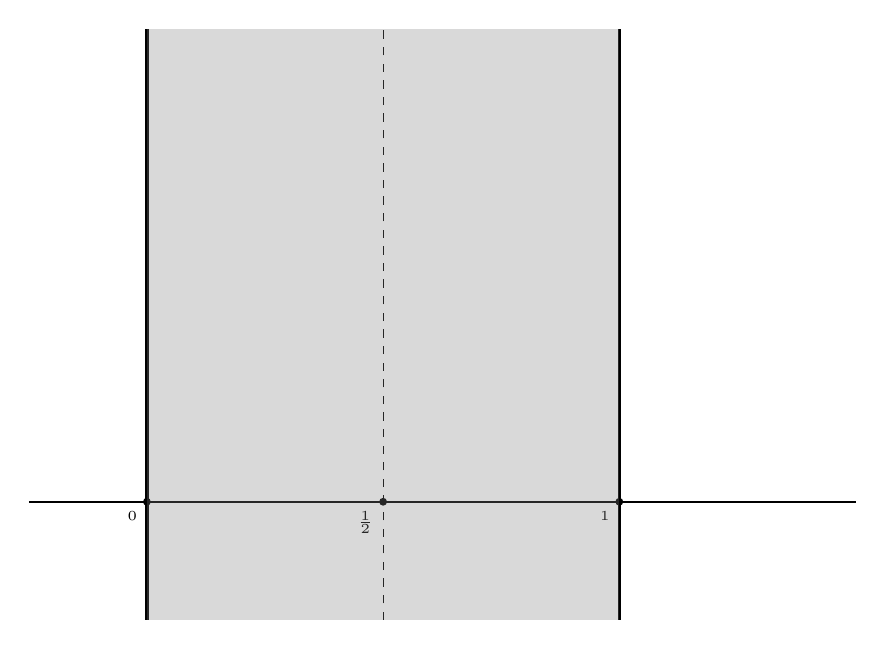
\begin{tikzpicture}[scale=3]
        \def\xmin{-0.5} \def\xmax{3}
        \def\ymin{-0.5} \def\ymax{2}
        \draw[thick] (\xmin,0) -- (\xmax,0);
        \draw[very thick] (0,\ymin) -- (0,\ymax);
        \draw[very thick] (2,\ymin) -- (2,\ymax);
        \draw[dashed] (1,\ymin) -- (1,\ymax);

        \node at (0,0) [below left] {\tiny{$0$}};
        \node at (0,0) [circle,fill,inner sep=1pt]{};
        \node at (1,0) [below left] {\tiny{$\frac{1}{2}$}};
        \node at (1,0) [circle,fill,inner sep=1pt]{};
        \node at (2,0) [below left] {\tiny{$1$}};
        \node at (2,0) [circle,fill,inner sep=1pt]{};

        \begin{scope}
          \path[clip] (0,\ymin) -- (0,\ymax) -- (2,\ymax) -- (2,\ymin) -- cycle;
          \fill[gray,opacity=0.3] (0,\ymin) rectangle (2,\ymax);
        \end{scope}
      \end{tikzpicture}
      \caption{The critical strip, critical line, and central point.}
      \label{fig:critical_strip}
    \end{figure}

    Lastly, we provide some bounds about gamma functions, gamma factors, and their logarithmic derivatives that will be extremely useful in the study of $L$-functions. Suppose $\s$ is bounded and $|t| > 1$. Then $s$ is bounded away from zero and by \cref{equ:weaker_Stirling_formula} we have the asymptotic
    \[
      \G(s) \sim \sqrt{2\pi}t^{\s-\frac{1}{2}}e^{-\frac{\pi}{2}|t|}.
    \]
    This gives the weaker estimates
    \[
      \G(s) \ll t^{\s-\frac{1}{2}}e^{-\frac{\pi}{2}|t|} \quad \text{and} \quad \frac{1}{\G(s)} \ll t^{\frac{1}{2}-\s}e^{\frac{\pi}{2}|t|},
    \]
    for $|t| > 1$. It is not hard to obtain estimates that holds in vertical strips. Suppose $s$ is in the vertical strip $a \le \s \le b$ and is distance $\e$ away from the poles of $\G(s)$. Then $\G(s)$ is bounded on the compact region $a \le \s \le b$ with $|t| \le 1$ provided $s$ is distance $\e$ away from the poles of $\G(s)$. It follows that the estimates
    \begin{equation}\label{equ:modified_gamma_estimates}
      \G(s) \ll_{\e} (|t|+1)^{\s-\frac{1}{2}}e^{-\frac{\pi}{2}|t|} \quad \text{and} \quad \frac{1}{\G(s)} \ll (|t|+1)^{\frac{1}{2}-\s}e^{\frac{\pi}{2}|t|},
    \end{equation}
    are valid in the vertical strip $a \le \s \le b$ provided $s$ is distance $\e$ away from the poles of $\G(s)$ in the former case. We immediately obtain the useful estimate
    \[
      \frac{\G(1-s)}{\G(s)} \ll_{\e} (|t|+1)^{1-2\s},
    \]
    valid in the vertical strip $a \le \s \le b$ provided $s$ is distance $\e$ away from the poles of $\G(1-s)$. Moreover, it easily follows from the definition of $\g(s,f)$ that the estimates
    \begin{equation}\label{equ:gamma_factor_analytic_conductor_estimate}
      \frac{\g(1-s,f)}{\g(s,f)} \ll_{\e} \mf{q}_{\infty}(s,f)^{\frac{1}{2}-\s} \quad \text{and} \quad q(f)^{\frac{1}{2}-s}\frac{\g(1-s,f)}{\g(s,f)} \ll_{\e} \mf{q}(s,f)^{\frac{1}{2}-\s},
    \end{equation}
    are valid in the vertical strip $a \le \s \le b$ provided $s$ is distance $\e$ away from the poles of $\g(1-s,f)$. There are analogous useful estimates for the digamma function as well. To derive them, suppose $\s$ is bounded and $|t| > 1$. Then $s$ is bounded away from zero, so making use of the formula $\frac{\G'}{\G}(s+1) = \frac{\G'}{\G}(s)+\frac{1}{s}$ if $\s < 0$, \cref{equ:approximtion_for_digamma} gives the estimate
    \[
      \frac{\G'}{\G}(s) \ll \log(s).
    \]
    We can also obtain estimates that holds in vertical strips. Suppose $s$ is in the vertical strip $a \le \s \le b$ and is distance $\e$ away from the poles of $\G(s)$. Then $\frac{\G'}{\G}(s)$ is bounded on the compact region $a \le \s \le b$ with $|t| \le 1$ provided $s$ is distance $\e$ away from the poles of $\G(s)$. It follows that the estimate
    \[
      \frac{\G'}{\G}(s) \ll_{\e} \log(|s|+1),
    \]
    is valid in the vertical strip $a \le \s \le b$ provided $s$ is distance $\e$ away from the poles of $\G(s)$. It follows from the definition of $\g(s,f)$ that the estimates
    \begin{equation}\label{equ:digamma_gamma_factor_analytic_conductor_estimate}
      \frac{\g'}{\g}(s,f) \ll_{\e} \log\mf{q}_{\infty}(s,f) \quad \text{and} \quad \log(q(f))+\frac{\g'}{\g}(s,f) \ll_{\e} \log\mf{q}(s,f),
    \end{equation}
    are valid in the vertical strip $a \le \s \le b$ provided $s$ is distance $\e$ away from the poles of $\g(s,f)$. 
  \section{The Approximate Functional Equation}
    If $L(s,f)$ is an $L$-function, then there is a formula which acts as a compromise between the functional equation for $L(s,f)$ and expressing $L(s,f)$ as a Dirichlet series. This formula is known as the approximate functional equation and it is important because it is valid inside of the critical strip and therefore can be used to obtain data about $L(s,f)$ in that region. First we use \cref{equ:gamma_factor_analytic_conductor_estimate} to show that $L(s,f)$ has polynomial growth in the $t$-aspect in vertical strips:

    \begin{proposition}\label{prop:L_function_bounded_in_vertical_strips}
      For any $L$-function $L(s,f)$ and $a < b$, $L(s,f)$ is of polynomial growth in the $t$-aspect in the vertical half-strip $a \le \s \le b$ with $|t| \ge 1$.
    \end{proposition}
    \begin{proof}
      On the one hand, for $\s > \max(1,b)$ we have $L(s,f) \ll 1$ on the line $\s = 1$ with $t \ge 1$. On the other hand, the functional equation and \cref{equ:gamma_factor_analytic_conductor_estimate} together imply
      \[
        L(s,f) \ll \mf{q}(s,f)^{\frac{1}{2}-\s}L(1-s,f).
      \]
      Clearly $\mf{q}(s,f)^{\frac{1}{2}-\s}$ is of polynomial growth in the $t$-aspect provided $\s$ is bounded. As $|\s| < \max(a,b)$, we see that $L(s,f)$ is also of polynomial growth in the $t$-aspect for $|t| \ge 1$. Moreover, this estimate also implies $L(s,f)$ is bounded on the line $t = 1$ since $\s$ is bounded. As $L(s,f)$ is holomorphic for $|t| \ge 1$ and of order $1$, we can apply the Phragm\'en-Lindel\"of convexity principle in this region (see \cref{append:The_Phragmen_Lindelof_Convexity_principle}) so that $L(s,f)$ is of polynomial growth in the $t$-aspect in the vertical half-strip $a \le \s \le b$ with $|t| \ge 1$.
    \end{proof}

    \cref{prop:L_function_bounded_in_vertical_strips} is a very important property that $L$-functions possess. It is usually used to estimate Perron type formulas. We can also use it to deduce the \textbf{approximate function equation}\index{approximate function equation}:

    \begin{theorem}[Approximate functional equation]
      Let $L(s,f)$ be an $L$-function, $\Phi(u)$ be an even holomorphic function bounded in the vertical strip $|\tau| < a+1$ for any $a > 1$ such that $\Phi(0) = 1$, and let $X > 0$. Then for $s$ in the critical strip, we have
      \[
        L(s,f) = \sum_{n \ge 1}\frac{a_{f}(n)}{n^{s}}V_{s}\left(\frac{n}{\sqrt{q(f)}X}\right)+\e(s,f)\sum_{n \ge 1}\frac{\conj{a_{f}(n)}}{n^{1-s}}V_{1-s}\left(\frac{nX}{\sqrt{q(f)}}\right)+\frac{R}{q(f)^{\frac{s}{2}}\g(s,f)},
      \]
      where $V_{s}(y)$ is the inverse Mellin transform defined by
      \[
        V_{s}(y) = \frac{1}{2\pi i}\int_{(a)}\frac{\g(s+u,f)}{\g(s,f)}\Phi(u)y^{-u}\frac{du}{u},
      \]
      and
      \[
        \e(s,f) = \e(f)q(f)^{\frac{1}{2}-s}\frac{\g(1-s,f)}{\g(s,f)}.
      \]
      Moreover, $R$ is zero if $\L(s,f)$ is entire, and otherwise
      \[
        R = \left(\Res_{u = 1-s}+\Res_{u = -s}\right)\frac{\L(s+u,f)\Phi(u)X^{u}}{u}.
      \]
    \end{theorem}
    \begin{proof}
      Let
      \[
        I(X,s,f) = \frac{1}{2\pi i}\int_{(a)}\L(s+u,f)\Phi(u)X^{u}\,\frac{du}{u}.
      \]
      $L(s,f)$ has polynomial growth in the $t$-aspect by \cref{prop:L_function_bounded_in_vertical_strips}. From \cref{equ:modified_gamma_estimates} we see that $\g(s+u,f)$ exhibits rapid decay. Since $\Phi(u)$ is bounded, it follows that the integrand exhibits rapid decay in a vertical strip containing $|\tau| \le a$. Therefore the integral is locally absolutely uniformly convergent. Moreover, we may shift the line of integration to $(-a)$. In doing so, we pass by a simple pole at $u = 0$ and possible poles at $u = 1-s$ and $u = -s$, giving
      \[
        I(X,s,f) = \frac{1}{2\pi i}\int_{(-a)}\L(s+u,f)\Phi(u)X^{u}\,\frac{du}{u}+\L(s,f)+R.
      \]
      Applying the functional equation to $\L(s+u,f)$ and performing the change of variables $u \to -u$, we obtain
      \[
        I(X,s,f) = -\e(f)I(X^{-1},1-s,\conj{f})+\L(s,f)-R,
      \]
      since $\Phi(u)$ is even. This equation is equivalent to
      \[
        \L(s,f) = I(X,s,f)+\e(f)I(X^{-1},1-s,\conj{f})+R.
      \]
      Since $\Re(s+u) > 1$, we can expand the $L$-function $L(s,f)$ inside of $I(X,s,f)$ as a Dirichlet series:
      \begin{align*}
        I(X,s,f) &= \frac{1}{2\pi i}\int_{(a)}\L(s+u,f)\Phi(u)X^{u}\,\frac{du}{u} \\
        &= \frac{1}{2\pi i}\int_{(a)}q(f)^{\frac{s+u}{2}}\g(s+u,f)L(s+u,f)\Phi(u)X^{u}\,\frac{du}{u} \\
        &= \frac{1}{2\pi i}\int_{(a)}\sum_{n \ge 1}\frac{a_{f}(n)}{n^{s+u}}q(f)^{\frac{s+u}{2}}\g(s+u,f)\Phi(u)X^{u}\,\frac{du}{u} \\
        &= \sum_{n \ge 1}\frac{1}{2\pi i}\int_{(a)}\frac{a_{f}(n)}{n^{s+u}}q(f)^{\frac{s+u}{2}}\g(s+u,f)\Phi(u)X^{u}\,\frac{du}{u} && \text{FT} \\
        &= q(f)^{\frac{s}{2}}\g(s,f)\sum_{n \ge 1}\frac{a_{f}(n)}{n^{s}}\frac{1}{2\pi i}\int_{(a)}\frac{\g(s+u,f)}{\g(s,f)}\Phi(u)\left(\frac{\sqrt{q(f)}X}{n}\right)^{u}\,\frac{du}{u} \\
        &= q(f)^{\frac{s}{2}}\g(s,f)\sum_{n \ge 1}\frac{a_{f}(n)}{n^{s}}V_{s}\left(\frac{n}{\sqrt{q(f)}X}\right).
      \end{align*}
      Performing the same computation for $I(X^{-1},1-s,\conj{f})$ and substituting in the results, we arrive at
      \[
        \L(s,f) = q(f)^{\frac{s}{2}}\g(s,f)\sum_{n \ge 1}\frac{a_{f}(n)}{n^{s}}V_{s}\left(\frac{n}{\sqrt{q(f)}X}\right)+\e(f)q(f)^{\frac{1-s}{2}}\g(1-s,f)\sum_{n \ge 1}\frac{a_{f}(n)}{n^{1-s}}V_{1-s}\left(\frac{nX}{\sqrt{q(f)}}\right)+R.
      \]
      Diving by $q(f)^{\frac{s}{2}}\g(s,f)$ completes the proof.
    \end{proof}

    The approximate functional equation was first developed by Hardy and Littlewood in the series \cite{hardyzeros1921,hardyapproximate1923,hardyapproximate1929}. The function $V_{s}(y)$ has the effect of smoothing out the two sums on the right-hand side of the approximate functional equation. In most cases, we will take
    \[
      \Phi(u) = \cos^{-4d_{f}M}\left(\frac{\pi u}{4M}\right),
    \]
    for an integer $M \ge 1$. Clearly $\Phi(u)$ holomorphic in the vertical strip $|\tau| < (2M-2)+1$, even, and satisfies $\Phi(0) = 1$. To see that it is bounded in this vertical strip, using the formula $\cos(\t) = \frac{e^{i\t}+e^{-i\t}}{2}$, we have
    \begin{equation}\label{equ:choice_for_V_decay_estimate}
     \cos^{-4d_{f}M}\left(\frac{\pi u}{4M}\right) = \left(\frac{e^{i\frac{\pi u}{4M}}+e^{-i\frac{\pi u}{4M}}}{2}\right)^{-4d_{f}M} \ll e^{-d_{f}\pi|r|},
    \end{equation}
    where in the estimate we have used the reverse triangle equality. It follows that $\Phi(u)$ exhibits rapid decay. With this choice of $ \Phi(u)$, we can prove a useful bound for $V_{s}(y)$:

    \begin{proposition}\label{prop:V_function_decay}
      Let $L(s,f)$ be an $L$-function, set $\Phi(u) = \cos^{-4d_{f}M}\left(\frac{\pi u}{4M}\right)$ for some integer $M \ge 1$, and let $V_{s}(y)$ be the inverse Mellin transform defined by
      \[
        V_{s}(y) = \frac{1}{2\pi i}\int_{(2M-2)}\frac{\g(s+u,f)}{\g(s,f)}\Phi(u)y^{-u}\frac{du}{u}.
      \]
      Then for $s$ in the critical strip, $V_{s}(y)$ satisfies the estimate
      \[
        V_{s}(y) \ll \left(1+\frac{y}{\sqrt{\mf{q}_{\infty}(s,f)}}\right)^{-M}.
      \]
    \end{proposition}
    \begin{proof}
      Suppose $0 \le \s \le \frac{1}{2}$ so that $\s-\frac{1}{2} \le 0$. Then from \cref{equ:modified_gamma_estimates} and the reverse triangle inequality, we deduce that
      \[
        \frac{\G(s+u)}{\G(s)} \ll \frac{(|t+r|+1)^{\s+\tau-\frac{1}{2}}}{(|t|+1)^{\s-\frac{1}{2}}}e^{\frac{\pi}{2}(|t|-|t+r|)} \ll (|t+r|+1)^{\tau}e^{\frac{\pi}{2}|r|}.
      \]
      From the definition of $\mf{q}(s,f)$, the above estimate implies
      \[
        \frac{\g(s+u,f)}{\g(s,f)} \ll \mf{q}_{\infty}(s,f)^{\frac{\tau}{2}}e^{d_{f}\frac{\pi}{2}|r|},
      \]
      for $s$ in the critical strip. By \cref{equ:choice_for_V_decay_estimate}, the integral defining $V_{s}(y)$ is locally absolutely uniformly convergent and we may shift the line of integration to $(M)$. In doing so, we do not pass by any poles and obtain
      \[
        V_{s}(y) = \frac{1}{2\pi i}\int_{(M)}\frac{\g(s+u,f)}{\g(s,f)}\Phi(u)y^{-u}\frac{du}{u} \\
      \]
      The fact that $u$ is bounded away from zero, \cref{equ:choice_for_V_decay_estimate}, and the estimate for the ratio of gamma factors, gives the first estimate in the following chain:
      \begin{align*}
        V_{s}(y) &= \frac{1}{2\pi i}\int_{(M)}\frac{\g(s+u,f)}{\g(s,f)}\Phi(u)y^{-u}\frac{du}{u} \\
        &\ll \int_{-\infty}^{\infty}\mf{q}_{\infty}(s,f)^{\frac{M}{2}}e^{-d_{f}\frac{\pi}{2}|r|}y^{-M}\,dr \\
        &\ll \int_{-\infty}^{\infty}\mf{q}_{\infty}(s,f)^{\frac{M}{2}}e^{-d_{f}\frac{\pi}{2}|r|}(1+y)^{-M}\,dr \\
        &\ll \int_{-\infty}^{\infty}e^{-\frac{\pi}{2}d_{f}|r|}\left(1+\frac{y}{\sqrt{\mf{q}_{\infty}(s,f)}}\right)^{-M}\,dr \\
        &\ll \left(1+\frac{y}{\sqrt{\mf{q}_{\infty}(s,f)}}\right)^{-M}\int_{-\infty}^{\infty}e^{-\frac{\pi}{2}d_{f}|r|}\,dr \\
        &\ll \left(1+\frac{y}{\sqrt{\mf{q}_{\infty}(s,f)}}\right)^{-M},
      \end{align*}
      where in the third and fourth lines we have used that $cy \ll (1+cy)$ for all $y \ge 0$ and any $c$ and the last line holds since the integrand exhibits rapid decay. This completes the proof.
    \end{proof}

    From \cref{prop:V_function_decay} we see that $V_{s}(y)$ is bounded for $y \ll_{\e} \mf{q}_{\infty}(s,f)^{\frac{1}{2}+\e}$ and then starts to exhibit polynomial decay that can be taken arbitrarily large. In a similar spirit to the approximate functional equation, a useful summation formula can be derived from the functional equation of each $L$-function:

    \begin{theorem}
      Let $\psi(y)$ be a bump function and let $\Psi(s)$ denote its Mellin transform. Then for any $L$-function $L(s,f)$, we have
      \[
        \sum_{n \ge 1}a_{f}(n)\psi(n) = \frac{\e(f)}{\sqrt{q(f)}}\sum_{n \ge 1}a_{\conj{f}}(n)\phi(n)+R\Psi(1),
      \]
      where $\phi(y)$ is the inverse Mellin transform defined by
      \[
        \phi(y) = \frac{1}{2\pi i}\int_{(a)}q(f)^{s}\frac{\g(s,f)}{\g(1-s,f)}y^{-s}\Psi(1-s)\,ds,
      \]
      for any $a > 1$. Moreover, $R$ is zero if $L(s,f)$ is entire, and otherwise
      \[
        R = \Res_{s = 1}L(s,f).
      \]
    \end{theorem}
    \begin{proof}
      By smoothed Perron's formula,
      \[
        \sum_{n \ge 1}a_{f}(n)\psi(n) = \frac{1}{2\pi i}\int_{(a)}L(s,f)\Psi(s)\,ds.
      \]
      By \cref{prop:smoothing_function_Mellin_inverse_vertical_strips,prop:L_function_bounded_in_vertical_strips}, the integrand has polynomial decay of arbitrarily larger order and therefore is locally absolutely uniformly convergent. Shifting the line of integration to $(1-a)$, we pass by a potential pole at $s = 1$ from $L(s,f)$ and obtain
      \[
        \sum_{n \ge 1}a_{f}(n)\psi(n) = \frac{1}{2\pi i}\int_{(1-a)}L(s,f)\Psi(s)\,ds+R\Psi(1).
      \]
      Applying the functional equation, we further have
      \[
        \sum_{n \ge 1}a_{f}(n)\psi(n) = \frac{1}{2\pi i}\int_{(1-a)}\e(f)q(f)^{\frac{1}{2}-s}\frac{\g(1-s,f)}{\g(s,f)}L(1-s,\conj{f})\Psi(s)\,ds+R\Psi(1).
      \]
      Performing the change of variables $s \to 1-s$ in this latter integral gives
      \[
        \sum_{n \ge 1}a_{f}(n)\psi(n) = \frac{1}{2\pi i}\int_{(a)}\e(f)q(f)^{s-\frac{1}{2}}\frac{\g(s,f)}{\g(1-s,f)}L(s,\conj{f})\Psi(1-s)\,ds+R\Psi(1).
      \]
      The proof is complete upon interchanging the sum over the Dirichlet series and the integral by Fubini's theorem and factoring out $\frac{\e(f)}{\sqrt{q(f)}}$.
    \end{proof}
  \section{The Riemann Hypothesis \& Nontrivial Zeros}
    The zeros of an $L$-function $L(s,f)$ have interesting behavior. Recall that
    \[
      L(s,f) = \prod_{p}(1-\a_{1}(p)p^{-s})^{-1}(1-\a_{2}(p)p^{-s})^{-1} \cdots (1-\a_{d_{f}}(p)p^{-s})^{-1},
    \]
    for $\s > 1$. This product vanishes if and only if one of its factors are zero. As $\s > 1$, this is impossible so that $L(s,f)$ has no zeros in this region. The functional equation will allow us to understand more about the zeros of $L(s,f)$. Rewrite the functional equation for $L(s,f)$ as
    \begin{equation}\label{equ:fun_eq_for_zeros}
      L(s,f) = \e(f)q(f)^{\frac{1}{2}-s}\frac{\g(1-s,f)}{\g(s,f)}L(1-s,\conj{f}).
    \end{equation}
    If $\s < 0$ then $L(1-s,\conj{f})$ is nonzero by our previous comments. Moreover, $\g(1-s,f)$ is holomorphic and nonzero in this region because $\Re(\k_{j}) > -1$. We conclude that poles of $\g(s,f)$ are zeros of $L(s,f)$ for $\s < 0$. Such a zero is called a \textbf{trivial zero}\index{trivial zero}. From the definition of $\g(s,f)$, they are all simple and of the form $s = -(\k_{j}+2n)$ for some local root at infinity $\k_{j}$ and some integer $n \ge 0$. Any other zero of $L(s,f)$ is called a \textbf{nontrivial zero}\index{nontrivial zero} and it lies inside of the critical strip (it may also be a pole of $\g(s,f)$). Now let $\rho$ be a nontrivial zero of $L(s,f)$. Note that $L(\conj{s},\conj{f}) = \conj{L(s,f)}$ for $\s > 1$ where $L(s,f)$ is defined by a Dirichlet series and thus for all $s$ by the identity theorem. It follows that $\conj{\rho}$ is a nontrivial zero of $L(s,\conj{f})$ an from the functional equation $1-\conj{\rho}$ is also a nontrivial zero of $L(s,f)$. In short, the nontrivial zeros occur in pairs:
    \[
      \rho \quad \text{and} \quad 1-\conj{\rho}.
    \]
    We can sometimes say more. If $L(s,f)$ takes real values for $s > 1$, the Schwarz reflection principle implies $L(\conj{s},f) = \conj{L(s,f)}$ and that $L(s,f)$ takes real values on the entire real axis save for the possible poles at $s = 0$ and $ s = 1$. We find that $\conj{\rho}$ and $1-\conj{\rho}$ are nontrivial zeros too and therefore the nontrivial zeros of $L(s,f)$ come in sets of four and are displayed in \cref{fig:symmetric_nontrivial_zeros}:
    \[
      \rho, \quad \conj{\rho}, \quad 1-\rho, \quad \text{and} \quad 1-\conj{\rho}.
    \]

    \begin{figure}[ht]
      \centering
      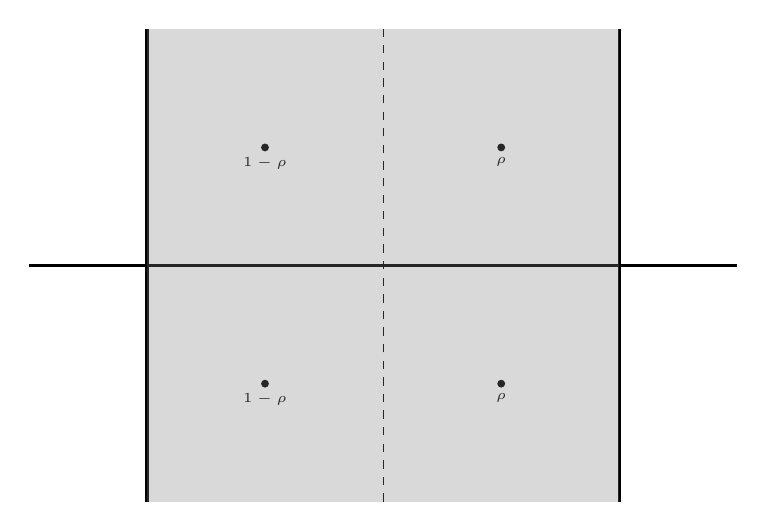
\begin{tikzpicture}[scale=3]
        \def\xmin{-0.5} \def\xmax{2.5}
        \def\ymin{-1} \def\ymax{1}
        \draw[thick] (\xmin,0) -- (\xmax,0);
        \draw[very thick] (0,\ymin) -- (0,\ymax);
        \draw[very thick] (2,\ymin) -- (2,\ymax);
        \draw[dashed] (1,\ymin) -- (1,\ymax);

        \node at (1.5,0.5) [circle,fill,inner sep=1pt]{};
        \node at (1.5,0.5) [below] {\tiny{$\rho$}};
        \node at (0.5,0.5) [circle,fill,inner sep=1pt]{};
        \node at (0.5,0.5) [below] {\tiny{$1-\conj{\rho}$}};
        \node at (1.5,-0.5) [circle,fill,inner sep=1pt]{};
        \node at (1.5,-0.5) [below] {\tiny{$\conj{\rho}$}};
        \node at (0.5,-0.5) [circle,fill,inner sep=1pt]{};
        \node at (0.5,-0.5) [below] {\tiny{$1-\rho$}};

        \begin{scope}
          \path[clip] (0,\ymin) -- (0,\ymax) -- (2,\ymax) -- (2,\ymin) -- cycle;
          \fill[gray,opacity=0.3] (0,\ymin) rectangle (2,\ymax);
        \end{scope}
        \end{tikzpicture}
      \caption{Symmetric nontrivial zeros.}
      \label{fig:symmetric_nontrivial_zeros}
    \end{figure}

    The \textbf{Riemann hypothesis}\index{Riemann hypothesis} for $L(s,f)$ says that this symmetry should be as simple as possible:

    \begin{conjecture}[Riemann hypothesis, $L(s,f)$ version]
      For the $L$-function $L(s,f)$, all of the nontrivial zeros lie on the line $\s = \frac{1}{2}$.
    \end{conjecture}

    Somewhat confusingly, do not expect the Riemann hypothesis to hold for just any $L$-function but we expect it to hold for many $L$-functions. In particular, the \textbf{grand Riemann hypothesis}\index{grand Riemann hypothesis} says that this symmetry should hold for any $L$-function in the Selberg class:

    \begin{conjecture}[Grand Riemann hypothesis]
      For any Selberg class $L$-function $L(s,f)$, all of the nontrivial zeros lie on the line $\s = \frac{1}{2}$.
    \end{conjecture}

    So far, the Riemann hypothesis remains completely out of reach for any $L$-function and thus the grand Riemann hypothesis does as well.
  \section{The Lindel\"of Hypothesis \& Convexity Bounds}
    Instead of asking about the zeros of an $L$-function $L(s,f)$ on the critical line, we can ask about the growth of $L(s,f)$, and more generally its derivatives, on the critical line. More precisely, we want to derive an upper bound for $L(s,f)$, or one of its derivatives, on the critical line using the Phragm\'en-Lindel\"of convexity principle. The argument we will describe for $L(s,f)$ is essentially a refinement of the proof of \cref{prop:L_function_bounded_in_vertical_strips}. Let
    \[
      p_{r_{f}}(s) = \left(\frac{s-1}{s+1}\right)^{r_{f}}.
    \]
    Note that $p_{r_{f}}(s) \sim 1$. The first step is to guarantee the Phragm\'en-Lindel\"of convexity principle for $p_{r_{f}}(s)L(s,f)$ in a region containing the critical strip. As $L(s,f)$ is of order $1$, this is assured (see \cref{append:The_Phragmen_Lindelof_Convexity_principle}). Therefore, we are reduced to estimating the growth of $p_{r_{f}}(s)L(s,f)$ for $\s$ to the left of $0$ and to the right of $1$. That is, just outside the edges of the critical strip. The right edge is easily estimated by setting $\s = 1+\e$ so that
    \[
      p_{r_{f}}(1+\e+it)L(1+\e+it,f) \ll_{\e} 1,
    \]
    which holds since $L(s,f)$ is defined by a locally absolutely uniformly convergent Dirichlet series for $\s > 1$. The left edge is only slightly more difficult. Upon isolating $L(s,f)$ in the functional equation, we have
    \[
      L(s,f) = \e(f)q(f)^{\frac{1}{2}-s}\frac{\g(1-s,f)}{\g(s,f)}L(1-s,f).
    \]
    Applying \cref{equ:gamma_factor_analytic_conductor_estimate} result in the bound
    \[
      L(s,f) \ll_{\e} \mf{q}(s,f)^{\frac{1}{2}-\s}L(1-s,f),
    \]
    for $s$ in any vertical strip with distance $\e$ away from the poles of $\g(1-s,f)$. Multiplying both sides by $p_{r_{f}}(s)$ and taking $\s = -\e$, it follows that
    \[
      p_{r_{f}}(-\e+it)L(-\e+it,f) \ll_{\e} \mf{q}(s,f)^{\frac{1}{2}+\e},
    \]
    which holds since $L(1-s,f)$ is defined by a locally absolutely uniformly convergent Dirichlet series for $\s < 0$. As $p_{r_{f}}(s)L(s,f)$ is holomorphic in a region containing the vertical strip $-\e \le \s \le 1+\e$ and $p_{r_{f}}(s) \sim 1$, the Phragm\'en-Lindel\"of convexity principle gives
    \begin{equation}\label{equ:convexity_bound_for_L_function_in_critial_strip}
      L(s,f) \ll_{\e} \mf{q}(s,f)^{\frac{1-\s}{2}+\e},
    \end{equation}
    in the vertical strip $-\e \le \s \le 1+\e$ provided $s$ is distance $\e$ away from the pole of $L(s,f)$ at $s = 1$ if it exists. At the critical line \cref{equ:convexity_bound_for_L_function_in_critial_strip} gives the following \textbf{convexity bound}\index{convexity bound}:
    \begin{equation}\label{equ:convexity_bound_L_function}
      L\left(\frac{1}{2}+it,f\right) \ll_{\e} \mf{q}\left(\frac{1}{2}+it,f\right)^{\frac{1}{4}+\e}.
    \end{equation}
    The \textbf{Lindel\"of hypothesis}\index{Lindel\"of hypothesis} for $L(s,f)$ says that the exponent can be reduced to $\e$:

    \begin{conjecture}[Lindel\"of hypothesis, $L(s,f)$ version]
      For the $L$-function $L(s,f)$, we have
      \[
        L\left(\frac{1}{2}+it,f\right) \ll_{\e} \mf{q}\left(\frac{1}{2}+it,f\right)^{\e}.
      \]
    \end{conjecture}

    Just as for the Riemann hypothesis, we do not expect the Lindel\"of hypothesis to hold for just any $L$-function. Accordingly, the \textbf{grand Lindel\"of hypothesis}\index{grand Lindel\"of hypothesis} says that the exponent can be reduced to $\e$ for any $L$-function in the Selberg class and we expect this to hold:

    \begin{conjecture}[Grand Lindel\"of hypothesis]
      For any Selberg class $L$-function $L(s,f)$, we have
      \[
        L\left(\frac{1}{2}+it,f\right) \ll_{\e} \mf{q}\left(\frac{1}{2}+it,f\right)^{\e}.
      \]
    \end{conjecture}

    Like the Riemann hypothesis, we have been unable to prove the Lindel\"of hypothesis for any $L$-function. However, the Lindel\"of hypothesis seems to be much more tractable. Generally speaking, any improvement upon the exponent in the convexity bound in any aspect of the analytic conductor is called a \textbf{subconvexity estimate}\index{subconvexity estimate} (or a \textbf{convexity breaking bound}\index{convexity breaking bound}). In other words, we would want a bound of the form
    \[
      L\left(\frac{1}{2}+it,f\right) \ll_{\e} \mf{q}\left(\frac{1}{2}+it,f\right)^{\d+\e},
    \]
    for some $0 \le \d \le \frac{1}{4}$. The convexity bound says that we may take $\d = \frac{1}{4}$ while the Lindel\"of hypothesis for $L(s,f)$ implies that we may take $\d = 0$.

    \begin{remark}
      Some subconvexity bounds are deserving of names. The cases $\d = \frac{3}{16}$ and $\d = \frac{1}{6}$ are referred to as the \textbf{Burgess bound}\index{Burgess bound} and \textbf{Weyl bound}\index{Weyl bound} respectively.
    \end{remark}
    
    With a little more work, we can obtain a a similar bound for $L^{(n)}(s,f)$ for any $n \ge 1$. First observe that \cref{equ:convexity_bound_for_L_function_in_critial_strip} implies
    \[
      L(s,f) \ll_{\e} \mf{q}\left(\frac{1}{2}+it,f\right)^{\frac{1}{4}+\e},
    \]
    in the vertical strip $\left|\s-\frac{1}{2}\right| \le \frac{\e}{2}$. This is just slightly stronger than the convexity bound. Now Cauchy's integral formula gives
    \[
      L^{(n)}\left(\frac{1}{2}+it,f\right) = \frac{n!}{2\pi i}\oint_{C}\frac{L(s,f)}{(s-\frac{1}{2}-it)^{n+1}}\,ds \ll_{\e} \oint_{C}|L(s,f)|ds,
    \]
    where $C$ is a circle about $\frac{1}{2}+it$ of radius $\frac{\e}{2}$. These two estimates, and that the disk bounded by $C$ is compact, together imply the following \textbf{convexity bound}\index{convexity bound}:
    \[
      L^{(n)}\left(\frac{1}{2}+it,f\right) \ll_{\e} \mf{q}\left(\frac{1}{2}+it,f\right)^{\frac{1}{4}+\e}.
    \]
  \section{Estimating the Central Value}
    The Lindel\"of hypothesis is concerned with the growth of the $L$-function $L(s,f)$ along the critical line, but sometimes we are only concerned with the size of $L(s,f)$ at the central point. The value of $L(s,f)$ at the central point is called the \textbf{central value}\index{central value} of $L(s,f)$. Many important properties about $L(s,f)$ can be connected to its central value. Any argument used to estimate the central value of an $L$-function is called a \textbf{central value estimate}\index{central value estimate}. We will prove central value estimate which gives a very useful upper bound in the $q(f)$-aspect. To state it, let $\psi(y)$ be a bump function with compact support in $\left[\frac{1}{2},2\right]$. For example,
    \[
      \psi(y) = \begin{cases} e^{-\frac{1}{9-(4y-5)^{2}}} & \text{if $|4y-5| < 3$}, \\ 0 & \text{if $|4y-5| \ge 3$}. \end{cases}
    \]
    The theorem is the following:

    \begin{theorem}
      Let $L(s,f)$ be an $L$-function and let $\psi(y)$ be a bump function with compact support in $\left[\frac{1}{2},2\right]$. Then we have
      \[
        L\left(\frac{1}{2},f\right) \ll_{\e} \max_{X \ll \mf{q}(f)^{\frac{1}{2}+\e}}\left(\left|\frac{A_{\psi}(X)}{q(f)^{\frac{1}{4}}}\right|\right)+\left|\frac{S}{q(f)^{\frac{1}{4}}}\right|,
      \]
      where $S$ is zero if $\L(s,f)$ is entire, and otherwise
      \[
        S = \left(\Res_{u = \frac{1}{2}}+\Res_{u = -\frac{1}{2}}\right)\L\left(\frac{1}{2}+u,f\right).
      \]
    \end{theorem}
    \begin{proof}
      Taking $s = \frac{1}{2}$, $X = 1$, and $\Phi(u) = \cos^{-4dM}\left(\frac{\pi u}{4M}\right)$ with $M \gg 1$ in the approximate functional equation gives
      \[
        L\left(\frac{1}{2},f\right) = \sum_{n \ge 1}\frac{a_{f}(n)}{\sqrt{n}}V_{\frac{1}{2}}\left(\frac{n}{\sqrt{q(f)}}\right)+\e(f)\sum_{n \ge 1}\frac{\conj{a_{f}(n)}}{\sqrt{n}}V_{\frac{1}{2}}\left(\frac{n}{\sqrt{q(f)}}\right)+\frac{R}{q(f)^{\frac{1}{4}}\g\left(\frac{1}{2},f\right)}.
      \]
      This implies the bound
      \[
        L\left(\frac{1}{2},f\right) \ll \left|\sum_{n \ge 1}\frac{a_{f}(n)}{\sqrt{n}}V_{\frac{1}{2}}\left(\frac{n}{\sqrt{q(f)}}\right)\right|+\left|\frac{S}{q(f)^{\frac{1}{4}}}\right|.
      \]
      Now consider the set of functions $\left\{\psi\left(\frac{y}{2^{k}}\right)\right\}_{k \in \Z}$. Since $\psi\left(\frac{y}{2^{k}}\right)$ has support in $[2^{k-1},2^{k+1}]$, the sum $\s(y) = \sum_{k \in \Z}\psi\left(\frac{y}{2^{k}}\right)$, defined for $y > 0$, is finite since at most finitely many terms are nonzero for every $y$. It is also bounded away from zero since for any $y > 0$ there is some $k \in \Z$ for which $2^{k} \le y \le 3 \cdot 2^{k-1}$ so that $\frac{y}{2^{k}}$ is at least distance $\frac{1}{2}$ from the endpoints of $\left[\frac{1}{2},2\right]$. Defining $\psi_{k}(y) = \psi\left(\frac{y}{2^{k}}\right)\s(y)^{-1}$, it follows that $\left\{\psi_{k}(y)\right\}_{k \in \Z}$ satisfies
      \[
        \sum_{k \in \Z}\psi_{k}(y) = 1,
      \]
      for any $y > 0$. Then we can write
      \[
        V_{s}(y) = \sum_{k \in \Z}\psi_{k}(y)V_{s}(y).
      \]
      It follows that
      \begin{align*}
        \sum_{n \ge 1}\frac{a_{f}(n)}{\sqrt{n}}V_{\frac{1}{2}}\left(\frac{n}{\sqrt{q(f)}}\right) &= \sum_{n \ge 1}\frac{a_{f}(n)}{\sqrt{n}}\sum_{k \in \Z}\psi_{k}\left(\frac{n}{\sqrt{q(f)}}\right)V_{\frac{1}{2}}\left(\frac{n}{\sqrt{q(f)}}\right) \\
        &= \sum_{k \in \Z}\sum_{n \ge 1}\frac{a_{f}(n)}{\sqrt{n}}\psi_{k}\left(\frac{n}{\sqrt{q(f)}}\right)V_{\frac{1}{2}}\left(\frac{n}{\sqrt{q(f)}}\right) && \text{FT} \\
        &\ll_{\e} \sum_{k \in \Z}\left|\sum_{\substack{n \ll \mf{q}(f)^{\frac{1}{2}+\e} \\ 2^{k-1}\sqrt{q(f)} \le n \le 2^{k+1}\sqrt{q(f)}}}\frac{a_{f}(n)}{\sqrt{n}}\psi_{k}\left(\frac{n}{\sqrt{q(f)}}\right)\right| \\
        &\ll_{\e} \sum_{k \ll \log(q(f)^{\frac{\e}{2}})}\left|\sum_{\substack{n \ll \mf{q}(f)^{\frac{1}{2}+\e} \\ 2^{k-1}\sqrt{q(f)} \le n \le 2^{k+1}\sqrt{q(f)}}}\frac{a_{f}(n)}{\sqrt{n}}\psi_{k}\left(\frac{n}{\sqrt{q(f)}}\right)\right|,
      \end{align*}
      where in the second to last line we have used that $V_{\frac{1}{2}}\left(\frac{n}{\sqrt{q(f)}}\right)$ is bounded for $n \ll_{\e} \mf{q}\left(\frac{1}{2},f\right)^{\frac{1}{2}+\e} \ll_{\e} \mf{q}(f)^{\frac{1}{2}+\e}$ and then exhibits polynomial decay thereafter by \cref{prop:V_function_decay} and in the last line we have used that $\psi_{k}(y)$ has compact support in $[2^{k-1},2^{k+1}]$ (recall $k \in \Z$). Since $\s(y)$ is bounded away from zero and $\log(y) \ll y$, we obtain the crude bound
      \[
        \sum_{k \ll \log(q(f)^{\frac{\e}{2}})}\left|\sum_{\substack{n \ll \mf{q}(f)^{\frac{1}{2}+\e} \\ 2^{k-1}\sqrt{q(f)} \le n \le 2^{k+1}\sqrt{q(f)}}}\frac{a_{f}(n)}{\sqrt{n}}\psi_{k}\left(\frac{n}{\sqrt{q(f)}}\right)\right| \ll_{\e} q(f)^{\frac{\e}{2}}\max_{X \ll \mf{q}(f)^{\frac{1}{2}+\e}}\left(\left|\sum_{\frac{X}{2} \le n \le 2X}\frac{a_{f}(n)}{\sqrt{n}}\psi\left(\frac{n}{X}\right)\right|\right).
      \]
      We will estimate this latter sum. Abel's summation formula (see \cref{{append:Summation_Formulas}}) gives
      \[
        \sum_{\frac{X}{2} \le n \le 2X}\frac{a_{f}(n)}{\sqrt{n}}\psi\left(\frac{n}{X}\right) = \frac{A_{\psi}(2X)}{\sqrt{2X}}-\frac{A_{\psi}\left(\frac{X}{2}\right)}{\sqrt{\frac{X}{2}}}+\frac{1}{2}\int_{\frac{X}{2}}^{2X}A_{\psi}(u)u^{-\frac{3}{2}}\,du.
      \]
      But as
      \[
        \frac{1}{2}\int_{\frac{X}{2}}^{2X}A_{\psi}(u)u^{-\frac{3}{2}}\,du \ll X\max_{\frac{X}{2} \le u \le 2X}\left(\left|A_{\psi}(u)u^{-\frac{3}{2}}\right|\right) \ll \max_{\frac{X}{2} \le u \le 2X}\left(\left|\frac{A_{\psi}(u)}{\sqrt{u}}\right|\right),
      \]
      we obtain the bound
      \[
        \max_{X \ll \mf{q}(f)^{\frac{1}{2}+\e}}\left(\left|\sum_{\frac{X}{2} \le n \le 2X}\frac{a_{f}(n)}{\sqrt{n}}\psi\left(\frac{n}{X}\right)\right|\right) \ll \max_{X \ll \mf{q}(f)^{\frac{1}{2}+\e}}\left(\left|\frac{A_{\psi}(X)}{\sqrt{X}}\right|\right).
      \]
      Putting everything together gives
      \[
        \sum_{n \ge 1}\frac{a_{f}(n)}{\sqrt{n}}V_{\frac{1}{2}}\left(\frac{n}{\sqrt{q(f)}}\right) \ll_{\e} q(f)^{\frac{\e}{2}}\max_{X \ll \mf{q}(f)^{\frac{1}{2}+\e}}\left(\left|\frac{A_{\psi}(X)}{\sqrt{X}}\right|\right) \ll_{\e} \max_{X \ll \mf{q}(f)^{\frac{1}{2}+\e}}\left(\left|\frac{A_{\psi}(X)}{q(f)^{\frac{1}{4}}}\right|\right),
      \]
      where in the last estimate we may replace $X$ with $q(f)^{\frac{1}{2}+\e}$ because $X \ge 1$ so that $X$ is bounded away from zero.
    \end{proof}
  \section{Logarithmic Derivatives}
    There is an incredibly useful formula for the logarithmic derivative of any $L$-function which is often the starting point for deeper analytic investigations. To deduce it, we will need a more complete understanding of $\L(s,f)$. First observe that the zeros $\rho$ of $\L(s,f)$ are contained inside of the critical strip. Indeed, we have already remarked that $L(s,f)$ has no zeros for $\s > 0$ and clearly $\g(s,f)$ does not have zeros in this region as well. Therefore $\L(s,f)$ is nonzero for $\s > 1$. By the functional equation, $\L(s,f)$ is also nonzero for $\s < 0$ too. In other words, the zeros of $\L(s,f)$ are the nontrivial zeros of $L(s,f)$. Before we state our result, we setup some notation. For an $L$-function $L(s,f)$ we define
    \[
      \xi(s,f) = (s(1-s))^{r_{f}}\L(s,f).
    \]
    Note that $\xi(s,f)$ is essentially just $\L(s,f)$ with the potential poles at $s = 0$ and $s = 1$ removed. From the functional equation, we also have
    \[
      \xi(s,f) = \e(f)\xi(1-s,\conj{f}).
    \]
    We now state our desired result:

    \begin{proposition}\label{prop:explicit_formula_log_derivative}
      For any $L$-function $L(s,f)$, there exist constants $A(f)$ and $B(f)$ such that
      \[
        \xi(s,f) = e^{A(f)+B(f)s}\prod_{\rho \neq 0,1}\left(1-\frac{s}{\rho}\right)e^{\frac{s}{\rho}},
      \]
      and hence the sum
      \[
        \sum_{\rho \neq 0,1}\frac{1}{|\rho|^{1+\e}},
      \]
      is convergent provided the product and sum are both counted with multiplicity and ordered with respect to the size of the ordinate. Moreover,
      \[
        -\frac{L'}{L}(s,f) = \frac{r_{f}}{s}+\frac{r_{f}}{s-1}+\frac{1}{2}\log{q(f)}+\frac{\g'}{\g}(s,f)-B(f)-\sum_{\rho \neq 0,1}\left(\frac{1}{s-\rho}+\frac{1}{\rho}\right).
      \] 
    \end{proposition}
    \begin{proof}
      For the first statement, observe that $\xi(s,f)$ is entire since the only possible poles of $\L(s,f)$ are at $s = 0$ and $s = 1$ and are of order $r_{f}$. We also claim that $\xi(s,f)$ is of order $1$. By the functional equation, it suffices to show this for $\s \ge \frac{1}{2}$. This follows from $L(s,f)$ being of order $1$ and \cref{equ:modified_gamma_estimates} (within $\e$ of the poles of $\g(s,f)$ we know $\xi(s,f)$ is bounded because it is entire). By the Hadamard factorization theorem (see \cref{append:Factorizations_and_Finite_Order}),
       \[
        \xi(s,f) = e^{A(f)+B(f)s}\prod_{\rho \neq 0,1}\left(1-\frac{s}{\rho}\right)e^{\frac{s}{\rho}},
      \]
      for some constants $A(f)$ and $B(f)$ and the desired sum converges. This proves the first statement. For the second, taking the logarithmic derivative of the definition of $\xi(s,f)$ yields
      \begin{equation}\label{equ:log_derivative_1}
        \frac{\xi'}{\xi}(s,f) = \frac{r_{f}}{s}+\frac{r_{f}}{s-1}+\frac{1}{2}\log{q(f)}+\frac{\g'}{\g}(s,f)+\frac{L'}{L}(s,f).
      \end{equation}
      On the other hand, taking the logarithmic derivative of the Hadamard factorization gives
      \begin{equation}\label{equ:log_derivative_2}
        \frac{\xi'}{\xi}(s,f) = B(f)+\sum_{\rho \neq 0,1}\left(\frac{1}{s-\rho}+\frac{1}{\rho}\right).
      \end{equation}
      Equating \cref{equ:log_derivative_1,equ:log_derivative_2}, we arrive at
      \[
        B(f)+\sum_{\rho \neq 0,1}\left(\frac{1}{s-\rho}+\frac{1}{\rho}\right) = \frac{r_{f}}{s}+\frac{r_{f}}{s-1}+\frac{1}{2}\log{q(f)}+\frac{\g'}{\g}(s,f)+\frac{L'}{L}(s,f).
      \]
      Isolating $-\frac{L'}{L}(s,f)$ completes the proof.
    \end{proof}

    We now need to make a few comments. Our first is regarding the constants $A(f)$ and $B(f)$. The explicit evaluation of these constants can be challenging and heavily depends upon the arithmetic object $f$. However, useful estimates are not too difficult to obtain. We also claim $A(\conj{f}) = \conj{A(f)}$ and $B(\conj{f}) = \conj{B(f)}$. To see this, recall that $L(\conj{s},\conj{f}) = \conj{L(s,f)}$. Then $\xi(\conj{s},\conj{f}) = \conj{\xi(s,f)}$ because $\g(s,\conj{f}) = \g(s,f)$, the $\k_{j}$ are real or occur in conjugate pairs, and $\G(\conj{s}) = \conj{\G(s)}$. But then the functional equation and \cref{prop:explicit_formula_log_derivative} together imply
    \[
      e^{A(\conj{f})+B(\conj{f})s} = \frac{\xi'}{\xi}(0,\conj{f}) = \conj{\frac{\xi'}{\xi}(0,f)} = e^{\conj{A(f)}+\conj{B(f)}s},
    \]
    and the claim follows. Our second comment concerns the negative logarithmic derivative of $L(s,f)$. In general, this function attracts much attention for analytic investigations. As $L(s,f)$ is holomorphic for $\s > 1$ and admits an Euler product there, we can take the logarithm of the Euler product (turning it into a sum) and differentiate termwise to obtain
    \begin{equation}\label{equ:log_derivaive_direct_computation}
      -\frac{L'}{L}(s,f) = -\sum_{p}\sum_{1 \le j \le d_{f}}\frac{d}{ds}\log(1-\a_{j}(p)p^{-s}) = \sum_{p}\sum_{1 \le j \le d_{f}}\frac{\a_{j}(p)\log(p)}{(1-\a_{j}(p)p^{-s})p^{s}}.
    \end{equation}
    From the Taylor series of $\frac{1}{1-s}$, it follows that $-\frac{L'}{L}(s,f)$ is a locally absolutely uniformly convergent Dirichlet series of the form
    \[
       -\frac{L'}{L}(s,f) = \sum_{n \ge 1}\frac{\L_{f}(n)}{n^{s}},
    \]
    for $\s > 1$, where
    \[
      \L_{f}(n) = \begin{cases} \sum_{1 \le j \le d_{f}}\a_{j}(p)^{k}\log(p) & \text{if $n = p^{k}$ for some $k \ge 1$}, \\ 0 & \text{otherwise}. \end{cases}
    \]
    It is worth noting that $\L_{\conj{f}}(n) = \conj{\L_{f}(n)}$.
  \section{Zero Density}
    The deepest subject of the theory of $L$-functions is arguably the distribution of the zeros of $L$-functions. Here we introduce a method of counting zeros of $L$-functions and gaining a very simple understanding of their density as a result. We first require an immensely useful lemma:

    \begin{lemma}\label{lem:powerful_L-function_approximation_lemma}
      Let $L(s,f)$ be an $L$-function. The following statements hold:
      \begin{enumerate}[label=(\roman*)]
        \item The constant $B(f)$ satisfies
        \[
          \Re(B(f)) = -\sum_{\rho \neq 0,1}\Re\left(\frac{1}{\rho}\right),
        \]
        where the sum is counted with multiplicity and ordered with respect to the size of the ordinate.
        \item For any $T \ge 0$, the number of nontrivial zeros $\rho = \b+i\g$ with $\rho \neq 0,1$ and such that $|T-\g| \le 1$ is $O(\log{\mf{q}(iT,f)})$.
        \item For $\s > 1$, we have
        \[
          \Re\left(\frac{1}{s-\rho}\right) > 0 \quad \text{and} \quad \Re\left(\frac{1}{s+\k_{j}}\right) > 0.
        \]
        \item We have
        \[
          -\frac{L'}{L}(s,f) = \frac{r_{f}}{s}+\frac{r_{f}}{s-1}-\sum_{|s+\k_{j}| < 1}\frac{1}{s+\k_{j}}-\sum_{\substack{|s-\rho| < 1 \\ \rho \neq 0,1}}\frac{1}{s-\rho}+O(\log{\mf{q}(s,f)}),
        \]
        for any $s$ in the vertical strip $-\frac{1}{2} \le \s \le 2$. Moreover, in this vertical strip we also have
        \[
          \Re\left(-\frac{L'}{L}(s,f)\right) \le \Re\left(\frac{r_{f}}{s}\right)+\Re\left(\frac{r_{f}}{s-1}\right)-\sum_{|s+\k_{j}| < 1}\Re\left(\frac{1}{s+\k_{j}}\right)-\sum_{\substack{|s-\rho| < 1 \\ \rho \neq 0,1}}\Re\left(\frac{1}{s-\rho}\right)+O(\log{\mf{q}(s,f)}),
        \]
        and we may discard any term in either sum if $1 < \s \le 2$.
      \end{enumerate}
    \end{lemma}
    \begin{proof}
      We will prove each statement separately.
      \begin{enumerate}[label=(\roman*)]
        \item To prove (i), first recall that  $B(\conj{f}) = \conj{B(f)}$. Then \cref{equ:log_derivative_2} and the functional equation together imply
        \[
          2\Re(B(f)) = B(f)+B(\conj{f}) = -\sum_{\rho \neq 0,1}\left(\frac{1}{s-\rho}+\frac{1}{1-s-\conj{\rho}}+\frac{1}{\rho}+\frac{1}{\conj{\rho}}\right),
        \]
        where we have made use of the fact that the nontrivial zeros occur is pairs $\rho$ and $1-\conj{\rho}$ where the latter is also a nontrivial zero of $L(1-s,\conj{f})$. Now fix $s$ such that it does not coincide with the ordinate of a nontrivial zero. Then $s$ is bounded away from all of the nontrivial zeros and it follows that $\frac{1}{(s-\rho)}+\frac{1}{(1-s-\conj{\rho})} \ll \frac{1}{\rho^{2}}$ and $\frac{1}{\rho}+\frac{1}{\conj{\rho}} \ll \frac{1}{\rho^{2}}$. Therefore the sums
        \[
          \sum_{\rho \neq 0,1}\left(\frac{1}{s-\rho}+\frac{1}{1-s-\conj{\rho}}\right) \quad \text{and} \quad \sum_{\rho \neq 0,1}\left(\frac{1}{\rho}+\frac{1}{\conj{\rho}}\right),
        \]
        converge absolutely by \cref{prop:explicit_formula_log_derivative} and so we can sum them separately. The first sum vanishes by again using the fact that the nontrivial zeros occur is pairs $\rho$ and $1-\conj{\rho}$. Thus
        \[
          2\Re(B(f)) = \sum_{\rho \neq 0,1}\left(\frac{1}{\rho}+\frac{1}{\conj{\rho}}\right) = -\sum_{\rho \neq 0,1}\Re\left(\frac{1}{\rho}\right),
        \]
        which gives (i).
        \item For (ii), we first bound two important quantities. For the first quantity, the definition of $\L_{f}(n)$ and that $|\a_{j}(p)| \le p$ together imply the weak bound $|\L_{f}(n)| \le d_{f}n\log(n)$. Then
        \begin{equation}\label{equ:log_derivative_bound_conductor}
          \frac{L'}{L}(s,f) \ll d_{f}\z'(s-1) \ll \log{\mf{q}(f)},
        \end{equation}
        provided $\s > 2$. For the second quantity, \cref{equ:digamma_gamma_factor_analytic_conductor_estimate} implies
        \begin{equation}\label{equ:log_conductor_gamma_factor_bound_analytic_conductor}
          \frac{1}{2}\log{q(f)}+\frac{\g'}{\g}(s,f) \ll \log{\mf{q}(s,f)},
        \end{equation}
        for $\s > 0$. Now fix $T \ge 0$ and let $s = 3+iT$. Taking the real part of the formula for the negative logarithmic derivative in \cref{prop:explicit_formula_log_derivative} and combining \cref{equ:log_derivative_bound_conductor,equ:log_conductor_gamma_factor_bound_analytic_conductor} with (i) results in
        \[
          \sum_{\rho \neq 0,1}\Re\left(\frac{1}{s-\rho}\right) \ll \log{\mf{q}(iT,f)}.
        \]
        But as
        \[
          \frac{2}{9+(T-\g)^{2}} \le \Re\left(\frac{1}{s-\rho}\right) \le \frac{3}{4+(T-\g)^{2}},
        \]
        we obtain
        \begin{equation}\label{equ_sum_of_nontrivial_zeros_log_analytic_conductor_bound}
          \sum_{\rho \neq 0,1}\frac{1}{1+(T-\g)^{2}} \ll \log{\mf{q}(iT,f)},
        \end{equation}
        which is stronger than the first statement of (ii) since all of the terms in the sum are positive. The second statement is also clear.
        \item For (iii), just observe that
        \[
          \Re\left(\frac{1}{s-\rho}\right) = \frac{\s-\b}{(\s-\b)^{2}+(t-
          g)^{2}} > 0 \quad \text{and} \quad \Re\left(\frac{1}{s+\k_{j}}\right) = \frac{\s+\Re(\k_{j})}{(\s+\Re(\k_{j}))^{2}+(t+\Im(\k_{j}))^{2}} > 0,
        \]
        where the first bound holds because $\b \le 1$ and the second bound holds because $\Re(\k_{j}) > -1$.
        \item To deduce (iv), let $s$ be such that $-\frac{1}{2} \le \s \le 2$. Using \cref{equ:log_derivative_bound_conductor}, we can write
        \[
          -\frac{L'}{L}(s,f) = -\frac{L'}{L}(s,f)+\frac{L'}{L}(3+it,f)+O(\log{\mf{q}(s,f)}).
        \]
        Applying the formula for the negative logarithmic derivative in \cref{prop:explicit_formula_log_derivative} to the two terms on the right-hand side and using \cref{equ:digamma_gamma_factor_analytic_conductor_estimate} for $\s > 0$, we get
        \[
          -\frac{L'}{L}(s,f) = \frac{r_{f}}{s}+\frac{r_{f}}{s-1}+\frac{\g'}{\g}(s,f)-\sum_{\rho \neq 0,1}\left(\frac{1}{s-\rho}-\frac{1}{3+it-\rho}\right)+O(\log{\mf{q}(s,f)}).
        \]
        We now estimate the remaining sum. Retain the first part of the terms for which $|s-\rho| < 1$. The contribution from the second part of these terms is $O(\log{\mf{q}(it,f)})$ by (ii). For those terms with $|s-\rho| \ge 1$, we have
        \[
          \left|\frac{1}{s-\rho}-\frac{1}{3+it-\rho}\right| \le \frac{3-\s}{(3-\b)^{2}+(t-\g)^{2}} \le \frac{3}{1+(t-\g)^{2}}.
        \]
        Therefore from \cref{equ_sum_of_nontrivial_zeros_log_analytic_conductor_bound}, the contribution of these terms is $O(\log{\mf{q}(it,f)})$ too. It follows that
        \[
          -\frac{L'}{L}(s,f) = \frac{r_{f}}{s}+\frac{r_{f}}{s-1}+\frac{\g'}{\g}(s,f)-\sum_{\substack{|s-\rho| < 1 \\ \rho \neq 0,1}}\frac{1}{s-\rho}+O(\log{\mf{q}(s,f)}).
        \]
        Applying $\frac{\G'}{\G}(s+1) = \frac{\G'}{\G}(s)+\frac{1}{s}$ to $\frac{\g'}{\g}(s,f)$ and using \cref{equ:digamma_gamma_factor_analytic_conductor_estimate} gives
        \[
          \frac{\g'}{\g}(s,f) = -\sum_{|s+\k_{j}| < 1}\frac{1}{s+\k_{j}}+O(\log{\mf{q}_{\infty}(s,f)}).
        \]
        Then we obtain
        \[
          -\frac{L'}{L}(s,f) = \frac{r_{f}}{s}+\frac{r_{f}}{s-1}-\sum_{|s+\k_{j}| < 1}\frac{1}{s+\k_{j}}-\sum_{\substack{|s-\rho| < 1 \\ \rho \neq 0,1}}\frac{1}{s-\rho}+O(\log{\mf{q}(s,f)}),
        \]
        which is the first statement of (iv). For second statement, tak the real part of this estimate and write it as
        \[
          \sum_{|s+\k_{j}| < 1}\Re\left(\frac{1}{s+\k_{j}}\right)+\sum_{\substack{|s-\rho| < 1 \\ \rho \neq 0,1}}\Re\left(\frac{1}{s-\rho}\right) \le \Re\left(-\frac{L'}{L}(s,f)\right)+\Re\left(\frac{r_{f}}{s}\right)+\Re\left(\frac{r_{f}}{s-1}\right)+O(\log{\mf{q}(s,f)}).
        \]
        Now observe that we can discard any of the terms in either sum provided $1 < \s \le 2$ by (iii).
      \end{enumerate}
    \end{proof}

    With \cref{lem:powerful_L-function_approximation_lemma} in hand, we can deduce a result which estimates the number of nontrivial zeros in a box. Accordingly, for any $T \ge 0$ we define
    \[
      N(T,f) = |\{\rho = \b+i\g \in \C:\text{$L(\rho,f) = 0$ with $0 \le \b \le 1$ and $|\g| \le T$}\}|.
    \]
    In other words, $N(T,f)$ is the number of nontrivial zeros of $L(s,f)$ with ordinate in $[-T,T]$. We will prove the following:

    \begin{theorem}\label{thm:zero_counting}
      For any $L$-function $L(s,f)$ and $T \ge 1$,
      \[
        N(T,f) = \frac{T}{\pi}\log\left(\frac{q(f)T^{d_{f}}}{(2\pi e)^{d_{f}}}\right)+O(\log{\mf{q}(iT,f)}).
      \]
    \end{theorem}
    \begin{proof}
      Let $T \ge 1$ and set
      \[
        N'(T,f) = \left|\{\rho = \b+i\g \in \C:\text{$L(\rho,f) = 0$ with $0 \le \b \le 1$ and $0 < \g \le T$}\}\right|.
      \]
      As the nontrivial zeros occur in pairs $\rho$ and $1-\conj{\rho}$ where the latter is also a nontrivial zero of $L(s,\conj{f})$, it follows that
      \[
        N(T,f) = N'(T,f)+N'(T,\conj{f})+O(\log{\mf{q}(f)}),
      \]
      where $O(\log{\mf{q}(f)})$ accounts for the possible real nontrivial zeros. There are finitely many such nontrivial zeros because the interval $0 \le s \le 1$ is compact. We will estimate $N'(T,f)$ and in doing so we may assume $L(s,f)$ does not vanish on the line $t = T$ by varying $T$ by a sufficiently small constant, if necessary, and observing that $N(T,f)$ is modified by a quantity of size $O(\log{\mf{q}(iT,f)})$ by \cref{lem:powerful_L-function_approximation_lemma} (i). Since the nontrivial zeros are isolated, let $\d > 0$ be small enough such that $\L(s,f)$ has no nontrivial zeros for $-\d \le t < 0$. Then by our previous comments and the argument principle,
      \[
        N'(T,f) = \frac{1}{2\pi i}\int_{\eta}\frac{\xi'}{\xi}(s,f)\,ds+O(\log{\mf{q}(iT,f)}),
      \]
      where $\eta = \sum_{1 \le i \le 6}\eta_{i}$ is the contour in \cref{fig:zero_counting_contour}:
      
      Since $\log(s) = \log{|s|}+i\arg(s)$, we have
      \[
        \frac{1}{2\pi i}\int_{\eta}\frac{\xi'}{\xi}(s,f)\,ds = \frac{1}{2\pi i}\int_{\eta}\frac{d}{ds}\log{|\xi(s,f)|}\,ds+\frac{1}{2\pi }\int_{\eta}\frac{d}{ds}\arg\xi(s,f)\,ds = \frac{1}{2\pi}\D_{\eta}\arg(\xi(s,f)),
      \]
      where the last equality holds by parameterizing the curve $\eta$ and noting that $\eta$ is closed so that the first integral vanishes. For convenience, set $\eta_{L} = \eta_{1}+\eta_{2}+\eta_{3}$ and $\eta_{R} = \eta_{4}+\eta_{5}+\eta_{6}$. Recall that we have already shown $\xi(\conj{s},\conj{f}) = \conj{(\xi(s,f))}$. Using this fact along with the functional equation and that $-\arg(s) = \arg(\conj{s})$, we compute
      \begin{align*}
        \D_{\eta_{L}}\arg(\xi(s,f)) &= \D_{\eta_{L}}\arg\left(\e(f)\xi(1-s,\conj{f})\right) \\
        &= -\D_{\conj{\eta_{R}}}\arg\left(\e(f)\xi(s,\conj{f})\right) \\
        &= \D_{\conj{\eta_{R}}}\arg\left(\conj{\e(f)}\xi(\conj{s},f)\right) \\
        &= \D_{\eta_{R}}\arg\left(\conj{\e(f)}\xi(s,f)\right) \\
        &= \D_{\eta_{R}}\arg\left(\conj{\e(f)}\right)+\D_{\eta_{R}}\arg(\xi(s,f)) \\
        &= \D_{\eta_{R}}\arg(\xi(s,f)).
      \end{align*}

      \begin{figure}[ht]
        \centering
        \begin{tikzpicture}[scale=3]
          \def\xmin{-1.5} \def\xmax{2.5}
          \def\ymin{-0.5} \def\ymax{2}
          \draw[thick] (\xmin,0) -- (\xmax,0);
          \draw[very thick] (0,\ymin) -- (0,\ymax);
          \draw[very thick] (1,\ymin) -- (1,\ymax);
          \draw[dashed] (0.5,\ymin) -- (0.5,\ymax);

          \draw[->-] (0.5,-0.1) -- (2,-0.1);
          \draw[->-] (2,-0.1) -- (2,1.5);
          \draw[->-] (2,1.5) -- (0.5,1.5);
          \draw[->-] (0.5,1.5) -- (-1,1.5);
          \draw[->-] (-1,1.5) -- (-1,-0.1);
          \draw[->-] (-1,-0.1) -- (0.5,-0.1);

          \node at (1.25,-0.1) [below] {\tiny{$\eta_{1}$}};
          \node at (2,0.7) [right] {\tiny{$\eta_{2}$}};
          \node at (1.25,1.5) [above] {\tiny{$\eta_{3}$}};
          \node at (-0.25,1.5) [above] {\tiny{$\eta_{4}$}};
          \node at (-1,0.7) [left] {\tiny{$\eta_{5}$}};
          \node at (-0.25,-0.1) [below] {\tiny{$\eta_{6}$}};

          \node at (2,-0.1) [circle,fill,inner sep=1pt]{};
          \node at (2,1.5) [circle,fill,inner sep=1pt]{};
          \node at (0.5,1.5) [circle,fill,inner sep=1pt]{};
          \node at (-1,1.5) [circle,fill,inner sep=1pt]{};
          \node at (-1,-0.1) [circle,fill,inner sep=1pt]{};
          \node at (0.5,-0.1) [circle,fill,inner sep=1pt]{};

          \node at (2,-0.1) [below] {\tiny{$3-i\d$}};
          \node at (2,1.5) [above] {\tiny{$3+iT$}};
          \node at (0.5,1.5) [above left] {\tiny{$\frac{1}{2}+iT$}};
          \node at (-1,1.5) [above] {\tiny{$-2+iT$}};
          \node at (-1,-0.1) [below] {\tiny{$-2-i\d$}};
          \node at (0.5,-0.1) [below left] {\tiny{$\frac{1}{2}-i\d$}};
        \end{tikzpicture}
        \caption{A zero counting contour.}
        \label{fig:zero_counting_contour}
      \end{figure}

      In other words, the change in argument along $\eta_{L}$ is equal to the change in argument along $\eta_{R}$ and so
      \[
        \frac{1}{2\pi i}\int_{\eta}\frac{\xi'}{\xi}(s,f)\,ds = \frac{1}{\pi}\D_{\eta_{L}}\arg\xi(s,f).
      \]
      Thus to estimate the integral, we estimate the change in argument along $\eta_{L}$ of each factor in
      \[
        \xi(s,f) = (s(1-s))^{r_{f}}q(f)^{\frac{s}{2}}\pi^{-\frac{d_{f}s}{2}}\prod_{1 \le j \le d_{f}}\G\left(\frac{s+\k_{j}}{2}\right)L(s,f).
      \]
      For the factor $(s(1-s))^{r_{f}}$, we first have
      \[
        \D_{\eta_{L}}\arg(s) = \arg(s)\bigg|_{\frac{1}{2}-i\d}^{\frac{1}{2}+iT} = \arg\left(\frac{1}{2}+iT\right)-\arg\left(\frac{1}{2}-i\d\right) = O\left(\frac{1}{T}\right),
      \]
      and
      \[
        \D_{\eta_{L}}\arg(1-s) = \arg(1-s)\bigg|_{\frac{1}{2}-i\d}^{\frac{1}{2}+iT} = \arg\left(\frac{1}{2}-iT\right)-\arg\left(\frac{1}{2}+i\d\right) = O\left(\frac{1}{T}\right),
      \]
      where in both computations we have used $\arg(s) = \tan^{-1}\left(\frac{t}{\s}\right) = \frac{\pi}{2}+O\left(\frac{1}{t}\right)$, provided $\s > 0$, which holds by the Laurent series of the inverse tangent. Combining these two bounds, we obtain
      \begin{equation}\label{equ:zero_counting_1}
        \D_{\eta_{L}}(s(1-s))^{r_{f}} = O\left(\frac{1}{T}\right).
      \end{equation}
      For the factor $q(f)^{\frac{s}{2}}$, we use that $\arg(s) = \Im(\log(s))$ and compute
      \begin{equation}\label{equ:zero_counting_2}
        \D_{\eta_{L}}\arg{q(f)^{\frac{s}{2}}} = \Im(\log{q(f)^{\frac{s}{2}}})\bigg|_{\frac{1}{2}-i\d}^{\frac{1}{2}+iT} = \log{q(f)}\left(\frac{T}{2}+\frac{\d}{2}\right) = \frac{T}{2}\log{q(f)}+O(1).
      \end{equation}
      For the factor $\pi^{-\frac{d_{f}s}{2}}$, we use that $\arg(s) = \Im(\log(s))$ and compute
      \begin{equation}\label{equ:zero_counting_3}
        \D_{\eta_{L}}\arg(\pi^{-\frac{d_{f}s}{2}}) = \Im(\log(\pi^{-\frac{d_{f}s}{2}}))\bigg|_{\frac{1}{2}-i\d}^{\frac{1}{2}+iT} = \log\left(\frac{1}{\pi^{d_{f}}}\right)\left(\frac{T}{2}+\frac{\d}{2}\right) = \frac{T}{2}\log\left(\frac{1}{\pi^{d_{f}}}\right)+O(1).
      \end{equation}
      For the factor $\prod_{1 \le j \le d_{f}}\G\left(\frac{s+\k_{j}}{2}\right)$, we first use \cref{equ:log_gamma_estimate} (valid since $T \ge 1$) and that $\arg(s) = \Im(\log(s))$ to obtain
      \begin{align*}
        \D_{\eta_{L}}\arg\G(s) &= \Im(\log\G(s))\bigg|_{\frac{1}{2}-i\d}^{\frac{1}{2}+iT} \\
        &= T\log\left|\frac{1}{2}+iT\right|-T+\d\log\left|\frac{1}{2}+i\d\right|-\d+O(1) \\
        &= T\log(T)-T+O(1) \\
        &= T\log\left(\frac{T}{e}\right)+O(1).
      \end{align*}
      It follows that
      \begin{equation}\label{equ:zero_counting_4}
        \D_{\eta_{L}}\arg\left(\prod_{1 \le j \le d_{f}}\G\left(\frac{s+\k_{j}}{2}\right)\right) = \frac{T}{2}\log\left(\frac{T^{d_{f}}}{(2e)^{d_{f}}}\right)+O(\log{\mf{q}(f)}).
      \end{equation}
      For the factor $L(s,f)$, note that
      \[
        \D_{\eta_{L}}\arg(L(s,f)) = \Im(\log{L(s,f)})\bigg|_{\frac{1}{2}-i\d}^{\frac{1}{2}+iT} = \Im\left(\int_{\eta_{L}}\frac{L'}{L}(s,f)\,ds\right).
      \]
      By \cref{equ:log_derivative_bound_conductor}, the integral is $O(\log{q(f)})$ on $\eta_{2}$. On $\eta_{1}$ and $\eta_{3}$, \cref{lem:powerful_L-function_approximation_lemma} (ii) and (iv) together imply that the integral is $O(\log{\mf{q}(iT,f)})$. It follows that
      \begin{equation}\label{equ:zero_counting_5}
        \D_{\eta_{L}}\arg(L(s,f)) = O(\log{\mf{q}(iT,f)}).
      \end{equation}
      Combining \cref{equ:zero_counting_1,equ:zero_counting_2,equ:zero_counting_3,equ:zero_counting_4,equ:zero_counting_5} results in
      \[
        \frac{1}{\pi}\D_{\eta_{L}}\arg\xi(s,f) = \frac{T}{2\pi}\log\left(\frac{T^{d_{f}}}{(2\pi e)^{d_{f}}}\right)+O(\log{\mf{q}(iT,f)}),
      \]
      and therefore
      \[
        N'(T,f) = \frac{T}{2\pi}\log\left(\frac{T^{d_{f}}}{(2\pi e)^{d_{f}}}\right)+O(\log{\mf{q}(iT,f)}),
      \]
      The claim follows immediately from this estimate and that the same exact estimate holds for $N'(T,\conj{f})$ by using the $L$-function $L(s,\conj{f})$.
    \end{proof}

    It is worth noting that the main term in the proof of \cref{thm:zero_counting} comes from the change in argument of $q(f)^{\frac{s}{2}}\g(s,f)$ along the vertical segment $\eta_{3}$ (equivalently $\eta_{4}$). Moreover, the contribution from $L(s,f)$ is only to the error term. This is a good example of how analytic information of an $L$-function is intrinsically connected to its gamma factor. Also, with \cref{thm:zero_counting} we can now derive our zero density estimate:

    \begin{corollary}\label{cor:zero_density}
      For and $L$-function $L(s,f)$ and $T \ge 1$,
      \[
        \frac{N(T,f)}{T} \sim \frac{1}{\pi}\log\left(\frac{q(f)T^{d_{f}}}{(2\pi e)^{d_{f}}}\right).
      \]
    \end{corollary}
    \begin{proof}
      From \cref{thm:zero_counting},
      \[
        \frac{N(T,f)}{T} = \frac{1}{\pi}\log\left(\frac{q(f)T^{d_{f}}}{(2\pi e)^{d_{f}}}\right)\left(1+O\left(\frac{\log{\mf{q}(iT,f)}}{\log\left(\frac{q(f)T^{d_{f}}}{(2\pi e)^{d_{f}}}\right)T}\right)\right) = \frac{1}{\pi}\log\left(\frac{q(f)T^{d_{f}}}{(2\pi e)^{d_{f}}}\right)\left(1+O\left(\frac{1}{T}\right)\right).
      \]
      Since $O\left(\frac{1}{T}\right) = o(1)$, the result follows.
    \end{proof}

    \cref{cor:zero_density} can be interpreted as saying that for large $T$ the density of $N(T,f)$ is approximately $\frac{1}{\pi}\log\left(\frac{q(f)T^{d_{f}}}{(2\pi e)^{d_{f}}}\right)$. Since this grows as $T \to \infty$, we see that the nontrivial zeros tend to accumulate farther up the critical strip with logarithmic growth. We can dispense with this accumulation. If $\rho = \b+i\g$ is a nontrivial zero of $L(s,f)$, then we call $\rho_{\text{unf}} = \b+i\w$ the \textbf{unfolded nontrivial zero}\index{unfolded nontrivial zero} corresponding to $\rho$ where
    \[
      \w = \frac{\g}{\pi}\log\left(\frac{q(f)|\g|^{d_{f}}}{(2\pi e)^{d_{f}}}\right).
    \]
    Now for any $W \ge 0$, define
    \[
      N_{\text{unf}}(W,f) = |\{\rho_{\text{unf}} = \b+i\w \in \C:\text{$L(\rho,f) = 0$ with $0 \le \b \le 1$ and $|\w| \le W$}\}|.
    \]
    In other words, $N_{\text{unf}}(T,f)$ is the number of unfolded nontrivial zeros of $L(s,f)$ with ordinate in $[-W,W]$. We then have the following well-known result:

    \begin{proposition}\label{prop:unfolded_zeros_are_evenly_spaced}
    For any $L$-function $L(s,f)$ and $W \ge \frac{1}{\pi}\log\left(\frac{q(f)}{(2\pi e)^{d_{f}}}\right)$,
    \[
      \frac{N_{\text{unf}}(W,f)}{W} \sim 1.
    \]
    \end{proposition}
    \begin{proof}
      Consider the function $f(t)$ defined by
      \[
        f(t) = \frac{t}{\pi}\log\left(\frac{q(f)|t|^{d_{f}}}{(2\pi e)^{d_{f}}}\right),
      \]
      for $t \in \R$. Sine $f(t)$ is a strictly increasing continuous function, it has an inverse $g(w)$ for $w \in \R$. It follows that $|\w| \le W$ if and only if $|\rho| \le g(W)$ and so $N_{\text{unf}}(W,f) = N(g(W),f)$. But by \cref{cor:zero_density} and that $g(w)$ is the inverse of $f(t)$, we have $N(g(W),f) \sim W$. It follows that
      \[
        N_{\text{unf}}(W,f) \sim W,
      \]
      which is equivalent to the claim.
    \end{proof}

    We interpret \cref{prop:unfolded_zeros_are_evenly_spaced} as saying that the unfolded nontrivial zeros are evenly spaced opposed to \cref{cor:zero_density} which says that they tend to accumulate up the critical strip.
  \section{A Zero-free Region}
    Although the Riemann hypothesis remains out of reach, some progress has been made to understand regions inside of the critical strip for which $L$-functions are nonzero except for possibly one real exception. Such regions are known as \textbf{zero-free regions}\index{zero-free regions} and there is great interest in improving the breadth of such regions. We will derive a standard zero-free region for any $L$-function under some mild assumptions. First a useful lemma:

    \begin{lemma}\label{lem:non-vanshing_at_1_lemma}
      Let $L(s,f)$ be an $L$-function such that $\Re(\L_{f}(n)) \ge 0$ provided $(n,q(f)) = 1$. Also suppose that $|\a_{j}(p)| \le \frac{p}{2}$ for ramified primes $p$. Then $L(1,f) \neq 0$ and hence $r_{f} \ge 0$. Moreover, there exists a constant $c > 0$ such that $L(s,f)$ has at most $r_{f}$ real zeros in the region
      \[
        \s \ge 1-\frac{c}{d_{f}(r_{f}+1)\log{\mf{q}(f)}}.
      \]
    \end{lemma}
    \begin{proof}
      Let $\b_{j}$ be a real nontrivial zero with $\frac{1}{2} \le \b_{j} \le 1$. There are finitely many $\b_{j}$ since they belong to the compact interval $\frac{1}{2} \le s \le 1$ so we have $1 \le j \le n$ for some $n \ge 1$. Letting $1 < \s \le 2$, and applying \cref{lem:powerful_L-function_approximation_lemma} (iv) while discarding all the terms except those corresponding to the nontrivial zeros $\b_{j}$, we obtain the inequality
      \[
        \sum_{1 \le j \le n}\frac{1}{\s-\b_{j}} < \frac{r_{f}}{\s-1}+\Re\left(\frac{L'}{L}(\s,f)\right)+O(\log{\mf{q}(f)}).
      \]
      To estimate $\Re\left(\frac{L'}{L}(\s,f)\right)$, we first note that as $\Re(\L_{f}(n)) \ge 0$ provided $(n,q(f)) = 1$ by assumption, the Dirichlet series of $\frac{L'^{(q(f))}}{L^{(q(f))}}(s,f)$ shows that
      \[
        \Re\left(\frac{L^{(q(f))'}}{L^{(q(f))}}(\s,f)\right) \le 0.
      \]
      This gives an estimate for the contribution of the local factors of $L(s,f)$ corresponding to unramified primes. For the contribution of the local factors corresponding to ramified primes, we use \cref{equ:log_derivaive_direct_computation} to compute
      \[
        \Re\left(\frac{L'_{q(f)}}{L_{q(f)}}(\s,f)\right) \le \left|\frac{L'_{q(f)}}{L_{q(f)}}(\s,f)\right| = \left|\sum_{p \mid q(f)}\sum_{1 \le j \le d_{f}}\frac{\a_{j}(p)\log(p)}{(1-\a_{j}(p)p^{-\s})p^{\s}}\right| \le d_{f}\sum_{p \mid q(f)}\log(p) \le d_{f}\log(q(f)),
      \]
      where in the second inequality we have made use of the assumption $|\a_{j}(p)| \le \frac{p}{2}$ for ramified primes $p$ to conclude that $\left|\frac{\a_{j}(p)}{(1-\a_{j}(p)p^{-\s})p^{\s}}\right| \le 1$. These estimates together imply
      \[
        \sum_{1 \le j \le n}\frac{1}{\s-\b_{j}} < \frac{r_{f}}{\s-1}+O(\log{d_{f}\mf{q}(f)}).
      \]
      From this inequality we see that $\b_{j} \neq 1$. For if some $\b_{j} = 1$, $r_{f} < 0$ and the right-hand side is negative for $\s$ sufficiently close to $1$ contradicting the positivity of the left-hand side. Thus $L(1,f) \neq 0$ and hence $r_{f} \ge 0$. As there are finitely many $\b_{j}$, there exists a $c > 0$ such that the $\b_{j}$ satisfy
      \[
        \b_{j} \ge 1-\frac{c}{d_{f}(r_{f}+1)\log{\mf{q}(f)}}.
      \]
      Setting $\s = 1+\frac{2c}{d_{f}\log{\mf{q}(f)}}$ and choosing $c$ smaller, if necessary, we guarantee $1 < \s \le 2$. Then the two inequalities above together imply
      \[
        \frac{nd_{f}\log{\mf{q}(f)}}{2c+\frac{c}{(r_{f}+1)}} < \left(\frac{r_{f}}{2c}+O(1)\right)d_{f}\log{\mf{q}(f)}.
      \]
      Isolating $n$, we see that
      \[
        n < r_{f}+\frac{r_{f}}{2(r_{f}+1)}+O(c),
      \]
      and taking $c$ smaller, if necessary, we have $n \le r_{f}$. As $L(s,f)$ is nonzero for $\s > 1$, it follows that there are at most $r_{f}$ real zeros satisfying
      \[
        \s \ge 1-\frac{c}{d_{f}(r_{f}+1)\log{\mf{q}(f)}}.
      \]
      This completes the proof.
    \end{proof}

    We can now prove our zero-free region result:

    \begin{theorem}\label{thm:zero_free_region_generic}
      Let $L(s,f)$ be an $L$-function with at most a simple pole at $s = 1$, $\Re(\L_{f}(n)) \ge 0$ provided $(n,q(f)) = 1$, and $|\a_{j}(p)| \le \frac{p}{2}$ for ramified primes $p$. Then there exists a constant $c > 0$ such that $L(s,f)$ has no zeros in the region
      \[
        \s \ge 1-\frac{c}{d_{f}^{2}\log(\mf{q}(f)(|t|+3))},
      \]
      except for possibly one simple real zero $\b_{f}$ with $\b_{f} < 1$ in the case $L(s,f)$ has a simple pole at $s = 1$.
    \end{theorem}
    \begin{proof}
      For $t \in \R$, let $L(s,g)$ be the $L$-function defined by
      \[
        L(s,g) = L^{3}(s,f)L^{3}(s,\conj{f})L^{4}(s+it,f)L^{4}(s+it,\conj{f})L(s+2it,f)L(s+2it,\conj{f}).
      \]
      Clearly $d_{g} = 16d_{f}$ and so $\mf{q}(g)$ satisfies
      \[
        \mf{q}(g) \le \mf{q}(f)^{6}\mf{q}(it,f)^{8}\mf{q}(2it,f)^{2} \le \mf{q}(f)^{16d_{f}}(|t|+3)^{10d_{f}} < (\mf{q}(f)(|t|+3))^{16d_{f}}.
      \]
      We claim that $\Re(\L_{g}(n)) \ge 0$ for $(n,q(f)) = 1$. To see this, let $p$ be an unramified prime. The local roots of $L(s,g)$ at $p$ are $\a_{j}(p)$ and $\conj{\a_{j}(p)}$ both with multiplicity three, $\a_{j}(p)p^{-it}$ and $\conj{\a_{j}(p)}p^{-it}$ both with multiplicity four, and $\a_{j}(p)p^{-2it}$ and $\conj{\a_{j}(p)}p^{-2it}$ both with multiplicity one. So for any $k \ge 1$, the sum of $k$-th powers of these local roots is
      \[
       \sum_{1 \le j \le d_{f}}\left(6\Re(\a_{j}(p)^{k})+8\Re(\a_{j}(p)^{k})p^{-kit}+2\Re(\a_{j}(p)^{k})p^{-2kit}\right).
      \]
      The real part of this expression is
      \[
         (6+8\cos\log(p^{kt})+2\cos\log(p^{2kt}))\Re(\L_{f}(p^{k})) = 4(1+\cos\log(p^{kt}))^{2}\Re(\L_{f}(p^{k})) \ge 0.
      \]
      where we have made use of the identity $3+4\cos(\t)+\cos(2\t) = 2(1+\cos(\t))^{2}$. It follows that $\Re(\L_{g}(n)) \ge 0$ for $(n,q(f)) = 1$. Therefore the conditions of \cref{lem:non-vanshing_at_1_lemma} are satisfied for $L(s,g)$. Now let $\rho = \b+i\g$ be a complex nontrivial zero of $L(s,f)$. Setting $t = \g$, $L(s,g)$ has a real nontrivial zero at $s = \b$ of order at least $8$ and a pole at $s = 1$ of order $6$. That is, $r_{g} = 6$. But \cref{lem:non-vanshing_at_1_lemma} implies that $L(s,g)$ can have at most $6$ real nontrivial zeros in the given region. Letting the constant for the region in \cref{lem:non-vanshing_at_1_lemma} be $c'$, it follows that $\b$ must satisfy
      \[
        \b < 1-\frac{c'}{d_{g}(r_{g}+1)\log{\mf{q}(g)}} < 1-\frac{c'}{1792d_{f}^{2}\log(\mf{q}(f)(|\g|+3))},
      \]
  
      Take $c = \frac{c'}{1792}$. Now let $\b$ be a real nontrivial zero of $L(s,f)$. Since $\Re(\L_{f}(n)) \ge 0$ and $L(s,f)$ has at most a simple pole at $s = 1$, \cref{lem:non-vanshing_at_1_lemma} implies, upon shrinking $c$ if necessary, that there is at most one simple real zero $\b_{f}$ in the desired region and it can only occur if $L(s,f)$ has a simple pole at $s = 1$. Note that if $b_{f}$ exists, then $\b_{f} < 1$ because $L(s,f)$ is nonzero for $\s > 1$ and has a simple pole at $s = 1$. This completes the proof.
    \end{proof}
    
    Some comments are in order. Since the zeros of $L(s,f)$ occur in pairs $\rho$ and $1-\conj{\rho}$, the zero-free region in \cref{thm:zero_free_region_generic} implies a symmetric zero-free region about the critical line with at most one real zero in each half as displayed in \cref{fig:symmetric_zero_free_region}. The possible simple zero $b_{f}$ in \cref{thm:zero_free_region_generic} is referred to as a \textbf{Siegel zero}\index{Siegel zero} (or \textbf{exceptional zero}\index{exceptional zero}). If $\b_{f}$ is a Siegel zero of $L(s,\chi)$, then $1-\b_{f}$ is also a real nontrivial zero of $L(s,\chi)$ since the nontrivial zeros occur in pairs (or sets of four in some cases we have discussed). This immediately implies that $\b_{f} > \frac{1}{2}$ for we cannot have $\b_{f} = \frac{1}{2}$ since the zero is simple and either $\b_{f}$ or $1-\b_{f}$ must be at least $\frac{1}{2}$. Such zeros are conjectured to not exist. In full generality, \cref{thm:zero_free_region_generic} is the best result that one can hope for. It is possible to obtain better zero-free regions in certain cases but this heavily depends upon the particular $L$-function of interest and hence the arithmetic object $f$ attached to $L(s,f)$. In many cases it is possible to augment the proof of \cref{thm:zero_free_region_generic} to make the constant $c$ effective and such results have important applications. If $L(s,f)$ is of Selberg class, the conclusion of \cref{thm:zero_free_region_generic} is expected to hold without the possibly of a Siegel zero since $L(s,f)$ is expected to satisfy the Riemann hypothesis. Nevertheless, we can often satisfy the assumptions of \cref{thm:zero_free_region_generic}. Indeed, if $\a_{i}(p) \ge 0$ then the assumptions are satisfied immediately. If not, since $|\a_{i}(p)| \le 1$ the assumptions will hold for $\z(s)L(s,f)$ provided $L(s,f)$ does not have a pole at $s = 1$. This is often possible to prove in practice since $L(s,f)$ is expected to be entire unless $\a_{i}(p) \ge 0$.

    \begin{figure}[ht]
      \centering
      \begin{tikzpicture}[scale=3]
        \def\xmin{-0.5} \def\xmax{2.5}
        \def\ymin{-1} \def\ymax{1}
        \draw[thick] (\xmin,0) -- (\xmax,0);
        \draw[very thick] (0,\ymin) -- (0,\ymax);
        \draw[very thick] (2,\ymin) -- (2,\ymax);
        \draw[dashed] (1,\ymin) -- (1,\ymax);

        \node at (1.7,0) [circle,fill,inner sep=1pt]{};
        \node at (1.7,0) [below] {\tiny{$\b_{f}$}};
        \node at (0.3,0) [circle,fill,inner sep=1pt]{};
        \node at (0.3,0) [below] {\tiny{$1-\b_{f}$}};

        \draw[domain=-1:1,variable=\y] plot({1.5-((0.3)/ln(3+abs(\y)))},\y);
        \draw[domain=-1:1,variable=\y] plot({0.5+((0.3)/ln(3+abs(\y)))},\y);

        \fill [gray,opacity=0.3,domain=-1:1,variable=\y]
        (1.5,1)
        -- (2,1) 
        -- (2,-1)
        -- (1.5,-1)
        -- plot({1.5-((0.3)/ln(3+abs(\y)))},\y)
        -- cycle;

        \fill [gray,opacity=0.3,domain=-1:1,variable=\y]
        (0.5, 1)
        -- (0,1) 
        -- (0,-1)
        -- (0,-1)
        -- plot({0.5+((0.3)/ln(3+abs(\y)))},\y)
        -- cycle;
        \end{tikzpicture}
      \caption{The symmetric zero-free region in \cref{thm:zero_free_region_generic}.}
      \label{fig:symmetric_zero_free_region}
    \end{figure}
  \section{The Explicit Formula}
    A formula somewhat analogous to the approximate functional equation can be derived for the negative logarithmic derivative of any $L$-function. This formula is called the \textbf{explicit formula}\index{explicit formula}:

    \begin{theorem}[Explict Formula]
      Let $\psi(y)$ be a bump function with compact support and let $\Psi(s)$ denote its Mellin transform. Set $\phi(y) = y^{-1}\psi(y^{-1})$ so that its Mellin transform satisfies $\Phi(s) = \Psi(1-s)$. Then for any $L$-function $L(s,f)$, we have
      \begin{align*}
        \sum_{n \ge 1}\left(\L_{f}(n)\psi(n)+\L_{\conj{f}}(n)\phi(n)\right) &= \psi(1)\log{q(f)}+r_{f}\Psi(1) \\
        &+ \frac{1}{2\pi i}\int_{\left(\frac{1}{2}\right)}\left(\frac{\g'}{\g}(s,f)+\frac{\g'}{\g}(1-s,\conj{f})\right)\Psi(s)\,ds-\sum_{\rho}\Psi(\rho),
      \end{align*}
      where the sum is counted with multiplicity and ordered with respect to the size of the ordinate.
    \end{theorem}
    \begin{proof}
      By smoothed Perron's formula, we have
      \[
        \sum_{n \ge 1}\L_{f}(n)\psi(n) = \frac{1}{2\pi i}\int_{(c)}-\frac{L'}{L}(s,f)\Phi(s)\,ds,
      \]
      for any $c > 1$. Since the trivial zeros are isolated, let $\d > 0$ be such that there are no trivial zeros in the vertical strip $-2\d \le \s < 0$. By \cref{prop:smoothing_function_Mellin_inverse_vertical_strips,prop:L_function_bounded_in_vertical_strips}, the integrand has polynomial decay of arbitrarily large order and therefore is locally absolutely uniformly convergent. Shifting the line of integration to $(-\d)$, we pass by simple poles at $s = 1$ and $s = \rho$ for every nontrivial zero $\rho$ obtaining
      \[
        \sum_{n \ge 1}\L_{f}(n)\psi(n) = r_{f}\Psi(1)-\sum_{\rho}\Psi(\rho)+\frac{1}{2\pi i}\int_{(-\d)}-\frac{L'}{L}(s,f)\Psi(s)\,ds.
      \]
      For the latter integral, the functional equation and that $q(\conj{f}) = q(f)$ together imply
      \[
        -\frac{L'}{L}(s,f) = \log{q(f)}+\frac{\g'}{\g}(s,f)+\frac{\g'}{\g}(1-s,\conj{f})+\frac{L'}{L}(1-s,\conj{f}).
      \]
      Thus
      \[
        \frac{1}{2\pi i}\int_{(-\d)}-\frac{L'}{L}(s,f)\Phi(s)\,ds = \frac{1}{2\pi i}\int_{(-\d)}\left(\log{q(f)}+\frac{\g'}{\g}(s,f)+\frac{\g'}{\g}(1-s,\conj{f})+\frac{L'}{L}(1-s,\conj{f})\right)\Psi(s)\,ds.
      \]
      The integral over the first term on the right-hand side is $\psi(1)\log{q(f)}$ by the Mellin inversion formula. As for the last term, smoothed Perron's formula and that $\Phi(s) = \Psi(1-s)$ together give
      \[
        \frac{1}{2\pi i}\int_{(-\d)}-\frac{L'}{L}(1-s,\conj{f})\Psi(s)\,ds = \sum_{n \ge 1}\L_{\conj{f}}(n)\phi(n).
      \]
      So altogether, we have
      \begin{align*}
        \sum_{n \ge 1}\left(\L_{f}(n)\psi(n)+\L_{\conj{f}}(n)\phi(n)\right) &= \psi(1)\log{q(f)}+r_{f}\Psi(1) \\
        &+ \frac{1}{2\pi i}\int_{(-\d)}\left(\frac{\g'}{\g}(s,f)+\frac{\g'}{\g}(1-s,\conj{f})\right)\Psi(s)\,ds-\sum_{\rho}\Psi(\rho).
      \end{align*}
      Lastly, we note that by \cref{equ:approximtion_for_digamma,prop:smoothing_function_Mellin_inverse_vertical_strips}, the remaining integrand has polynomial decay of arbitrarily large order and therefore is locally absolutely uniformly convergent. Shifting the line of integration to $\left(\frac{1}{2}\right)$, we pass over no poles because the residues of $\frac{\g'}{\g}(1-s,\conj{f})$ are negative of those of $\frac{\g'}{\g}(s,f)$ for $\s \ge -\d$ (the nontrivial zeros of $L(s,f)$ occur in pairs $\rho$ and $1-\conj{\rho}$). This completes the proof. 
    \end{proof}

    The explicit formula is a very useful tool for analytic investigations. Since $\L_{f}(n)$ is essentially a weighted sum over prime powers, the explicit formula can be thought of as expressing a smoothed weighted sum over primes for $f$ in terms of the zeros of $L(s,f)$.